\documentclass[11pt]{article}
\usepackage[review]{acl}
\usepackage{times}
\usepackage{latexsym}
\usepackage[T1]{fontenc}
\usepackage[utf8]{inputenc}
\usepackage{microtype}
%\usepackage{inconsolata}
\usepackage{graphicx}
% ===== Additional packages =====
\usepackage{amsmath,amssymb}
\usepackage{amsthm}
\newtheorem{definition}{Definition}
\newtheorem{theorem}{Theorem}
\newtheorem{proposition}{Proposition}
\newtheorem{corollary}{Corollary}
\newtheorem*{remark}{Remark}
\usepackage{enumitem}
\usepackage{booktabs}
\usepackage{multirow}
\usepackage{xcolor}
\usepackage{colortbl}
\usepackage{hyperref}
\usepackage{cleveref}
% ===== Custom commands =====
\definecolor{cellbest}{HTML}{E8F4FD}
\definecolor{cellweak}{HTML}{FDE8E8}
\newcommand{\spm}[1]{{\scriptsize$\pm$#1}}
\newcommand{\spmg}[1]{{\color{gray}\scriptsize$\pm$#1}}

\title{From Specification to Causal Verification:\\ Do Transformers Implement Formally Prescribed Algorithms for Syntax?}

\author{Anonymous}

\begin{document}
\maketitle

%% ============================================================
%%  ABSTRACT
%% ============================================================
\begin{abstract}
Formal language theory tells us what Transformers \emph{can} compute; behavioral evaluation tells us what they \emph{get right}.
Neither tells us \emph{how}: whether a model that answers correctly does so by executing the algorithm that theory prescribes, or by exploiting surface shortcuts.
Bridging this gap would connect expressibility theory to mechanistic interpretability through a shared formal language.
%
We propose such a bridge.
We show that B-RASP, the programming language that exactly characterizes masked-hard-attention Transformer expressibility, can generate falsifiable causal hypotheses about model internals.
For four core English syntactic constraints (\textit{subject--verb agreement}, \textit{negative polarity item licensing}, \textit{reflexive binding}, and \textit{determiner--noun concord}), we write B-RASP programs specifying the prescribed algorithm, compile each into a structural causal model, and causally verify whether Transformers encode the prescribed intermediate variables.
%
From-scratch Transformers achieve near-perfect alignment with all four specifications (Interchange Intervention Accuracy, IIA $\geq$ 0.95), and pre-trained models show strong but imperfect alignment (0.82--0.95), with prescribed variables emerging during training in causal-dependency order.
This framework also reveals a structural limit of sparse autoencoder features on Boolean compositions and a widening Transformer-Mamba gap on long-distance dependencies.\footnote{Code and data are available at: \url{https://anonymous.4open.science/r/spec2verify}}
\end{abstract}

%% ============================================================
%%  INTRODUCTION
%% ============================================================
\section{Introduction}
\label{sec:intro}

Consider the sentence \textit{The keys to the cabinet are on the table}.
A competent English speaker knows that \textit{are} agrees with \textit{keys}, not with the linearly closer noun \textit{cabinet}, because agreement is governed by hierarchical structure, not linear proximity.
Three largely independent research programs bear on whether neural language models capture such dependencies, yet a basic question that sits at their intersection has not been answered.
Figure~\ref{fig:pipeline} previews our approach: we write a B-RASP program \citep{DBLP:conf/nips/Yang0A24} for the phenomenon, compile it into a Structural Causal Model \citep[SCM;][]{pearl2009causality}, and verify via Distributed Alignment Search \citep[DAS;][]{DBLP:conf/clear2/GeigerWPIG24} whether the prescribed variables are causally encoded in the network.

\begin{figure*}[t]
  \centering
  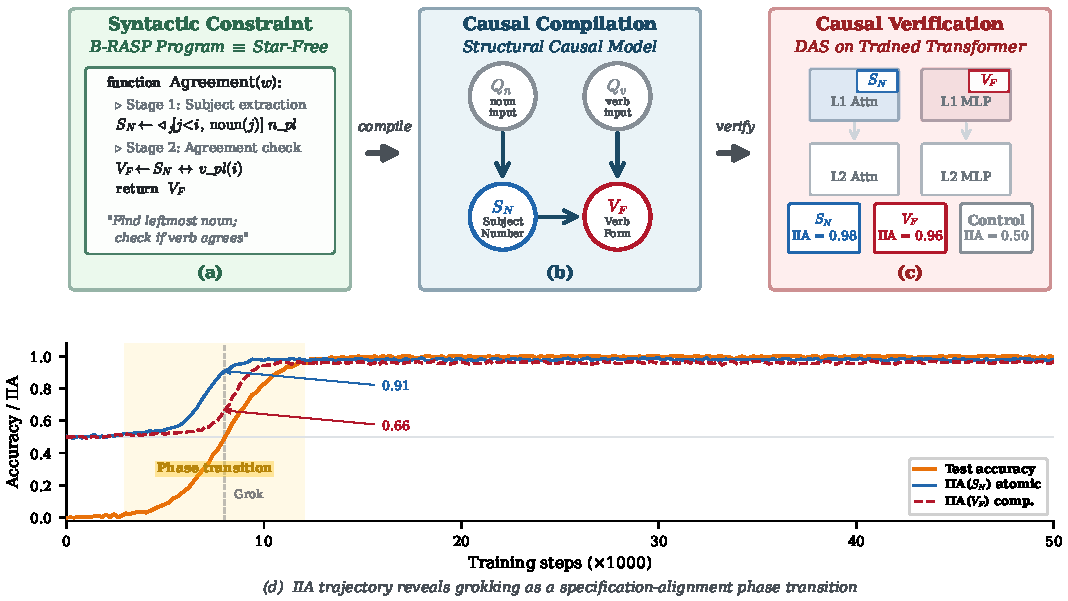
\includegraphics[width=0.87\textwidth]{figures/fig_pipeline.pdf}
  \caption{Overview of the specification-to-verification pipeline, illustrated with subject--verb agreement. \textbf{(a)}~A syntactic constraint is formalized as a B-RASP program \citep{DBLP:conf/nips/Yang0A24}. \textbf{(b)}~The program compiles into a structural causal model (SCM; \citealp{pearl2009causality}) whose variables (\textsc{subj\_num}, \textsc{verb\_form}) correspond to prescribed intermediate computations. \textbf{(c)}~DAS \citep{DBLP:conf/clear2/GeigerWPIG24} causally verifies whether each variable is encoded in the Transformer's activations, quantified by IIA. \textbf{(d)}~During training, the atomic variable \textsc{subj\_num} aligns before the compositional variable \textsc{verb\_form}, revealing grokking as a specification-alignment phase transition.}
  \label{fig:pipeline}
\end{figure*}

\paragraph{What Transformers can express.}
\citet{DBLP:conf/icml/WeissGY21} introduced RASP, a programming language whose select-aggregate-pointwise primitives mirror the operations of Transformer layers.
\citet{DBLP:conf/nips/Yang0A24} restricted RASP to Boolean values and proved that the resulting language, B-RASP, characterizes the expressibility of masked hard-attention Transformers exactly: the class of languages they recognize is the star-free regular languages, a well-studied subclass of the regular languages in which no unbounded counting is required \citep{mcnaughton1971counter}.
\citet{DBLP:journals/corr/abs-2510-19315} then established a succinctness gap: a B-RASP program of constant size can encode patterns whose smallest equivalent finite-state recognizer is exponentially large (see \citealp{DBLP:journals/tacl/StroblMW0A24} for a survey).
These results tell us what Transformers \emph{can} compute.
They do not tell us what a trained model \emph{actually} computes.

\paragraph{What trained models get right.}
\citet{linzen2016assessing} established the paradigm of probing subject--verb agreement with intervening \emph{attractors} (nouns whose grammatical number differs from the subject's), showing that LSTMs degrade as attractors accumulate.
Subsequent work scaled this paradigm to 67 minimal-pair contrasts spanning agreement, negative polarity items (NPIs), binding, and determiner--noun concord \citep{marvin2018targeted,warstadt2020blimp}, and demonstrated that architectural inductive bias matters more than dataset size for syntactic generalization \citep{hu2020systematic}.
These behavioral studies tell us \emph{that} models succeed or fail on particular constructions.
They do not tell us \emph{why}: a model can assign the correct verb form by relying on collocational shortcuts rather than hierarchical structure \citep{DBLP:journals/natmi/GeirhosJMZBBW20,DBLP:conf/acl/BhattamishraPKB23}.

\paragraph{The can-right-how gap.}
Expressibility establishes that a B-RASP program for agreement \emph{can} be compiled into Transformer weights.
Behavioral accuracy establishes that the model \emph{does} produce the correct verb form.
Neither establishes that the model follows the prescribed computational path: computing the subject's number, detecting interfering attractors, and composing these intermediate results into a verb-form decision.
Bridging this gap requires a causal methodology that tests whether a trained network faithfully realizes prescribed intermediate variables.\looseness=-1

\paragraph{Causal verification.}
The theory of causal abstraction \citep{DBLP:journals/jmlr/GeigerIZCC0AWGP25} provides such a methodology.
A high-level causal model is a faithful abstraction of a neural network when, for every \emph{interchange intervention} that sets a high-level variable to the value it would take under a different input, applying the corresponding intervention to aligned neural representations produces the same output change.
The fraction of such interventions that succeed is the Interchange Intervention Accuracy (IIA).
Distributed Alignment Search (DAS) learns the alignment by optimizing an orthogonal rotation of the residual stream via gradient descent, replacing brute-force search over neuron subsets.
Subsequent work has scaled DAS to billion-parameter models \citep{DBLP:conf/nips/WuGIPG23}, automated feature localization with hypernetworks \citep{DBLP:conf/iclr/Sun0BDPSG25}, and benchmarked it against alternative methods \citep{DBLP:conf/acl/HuangWPGG24,DBLP:conf/icml/MuellerGWAABCFH25}.
A recurring finding is that Sparse Autoencoder (SAE) features perform no better than raw neurons for causal variable localization \citep{DBLP:conf/icml/MuellerGWAABCFH25}, a result that lacks structural explanation.

All prior applications of causal abstraction, however, test hypotheses that researchers formulate by hand for each task.
We observe that B-RASP programs offer a principled alternative: because B-RASP provably characterizes masked hard-attention Transformer expressibility, compiling a B-RASP program into a SCM yields a causal hypothesis that is grounded in the same formalism, not in the researcher's intuition.

\paragraph{Methodological safeguards.}
Three recent critiques inform our experimental design.
Unconstrained alignment maps can make IIA vacuously high even for random networks \citep{sutter2025nonlinear}; subspace patching inside MLP layers can activate dormant pathways \citep{DBLP:conf/iclr/MakelovLGN24}; and multiple incompatible explanations can all achieve perfect IIA \citep{DBLP:conf/iclr/MelouxMPP25}.
We address these risks by restricting DAS to low-rank orthogonal rotations of the residual stream, by running negative controls (wrong SCM and random initialization both yield chance-level IIA), and by anchoring our specifications in formal language theory rather than in post-hoc reverse engineering.

Our goal is to test one formally specified reference algorithm per phenomenon, not to claim that it is the model's unique internal solution.

\paragraph{Contributions.}
\begin{enumerate}[itemsep=2pt,topsep=3pt,leftmargin=*]
    \item We compile B-RASP programs for four syntactic phenomena into SCMs and verify via DAS that all prescribed variables are strongly aligned ($\mathrm{IIA} \geq 0.95$ after grokking in from-scratch Transformers; $0.82$--$0.95$ across pre-trained Pythia and Llama-3.2 models).
    \item We show that prescribed variables emerge during grokking \citep[delayed generalization;][]{DBLP:journals/corr/abs-2201-02177} in causal-dependency order, yielding a specification-aligned progress measure that identifies \emph{which} variable is being acquired, unlike prior measures based on Fourier coefficients \citep{DBLP:conf/iclr/NandaCLSS23} or information-theoretic quantities \citep{DBLP:journals/corr/abs-2408-08944}.
    \item We explain why unsupervised feature decomposition falls short of supervised methods for causal variable localization: SAE features recover atomic variables (e.g., subject number) but degrade on compositional ones (e.g., verb-form agreement), because Boolean compositions lack a sparse basis that dictionary learning can recover \citep{DBLP:journals/corr/abs-2209-10652}.
    \item We observe a widening accuracy gap between Transformers and sequential models (Mamba, LSTM) on long-distance dependencies, consistent with the succinctness perspective: Transformers implement B-RASP programs in constant depth, while sequential models suffer from state interference as attractors accumulate.
\end{enumerate}

%% ============================================================
%%  §2 BACKGROUND
%% ============================================================
\section{Preliminaries}
\label{sec:prelim}

\subsection{Boolean RASP}
\label{sec:brasp}

A B-RASP program \citep{DBLP:conf/nips/Yang0A24} operates on an input string $w = w_1 \cdots w_n \in \Sigma^+$ and produces a Boolean output at a designated position.
The program manipulates \emph{Boolean vectors} $P \in \{0,1\}^n$, one entry per position.
The initial vectors $\{Q_\sigma\}_{\sigma \in \Sigma}$ encode the input: $Q_\sigma(i) = 1$ iff $w_i = \sigma$.
A program is a sequence of operations $t = 1, 2, \ldots$, each producing a new Boolean vector $P_t$ from those previously computed via one of two operation types: \textbf{(i) Pointwise.} $P_{t+1}(i) {:=}\; f\!\bigl(P_1(i), \ldots, P_t(i)\bigr)$ for an arbitrary Boolean function $f$, applied independently at every position $i$. \textbf{(ii) Attention.} $P_{t+1}(i) {:=}\; \triangleleft_j\bigl[M(i,j),\; S(i,j)\bigr]\; V\!(i,j) : D(i)$ selects the leftmost unmasked position $j$ maximizing a Boolean predicate $S$ and returns value $V\!(i,j)$ (or default $D(i)$ if no position is unmasked). Full semantics appear in Appendix~\ref{app:brasp}.
Each B-RASP operation compiles into one masked hard-attention Transformer layer, so program length upper-bounds the required depth.
Full formal definitions appear in Appendix~\ref{app:brasp}.

\subsection{Causal Abstraction and IIA}
\label{sec:causal-abstraction}

We formalize prescribed algorithms as structural causal models (SCMs; \citealp{pearl2009causality}).
An SCM $\mathcal{C} = (\mathbf{V}, \mathbf{F})$ consists of variables $\mathbf{V} = \mathbf{V}_{\mathrm{in}} \cup \mathbf{V}_{\mathrm{end}}$ (inputs and endogenous variables) and structural equations $\mathbf{F} = \{F_U\}_{U \in \mathbf{V}_{\mathrm{end}}}$, where $F_U$ computes the value of $U$ from its parents.

To test whether a neural network $\mathcal{N}$ faithfully implements $\mathcal{C}$, we define an \emph{alignment} $\tau$ that maps each $U \in \mathbf{V}_{\mathrm{end}}$ to a subspace of $\mathcal{N}$'s activations.
For a base input $\mathbf{b}$ and a source input $\mathbf{s}$, an \emph{interchange intervention} on $U$ proceeds in parallel:
in $\mathcal{C}$, the value of $U$ is set to the value it takes under $\mathbf{s}$;
in $\mathcal{N}$, the activations in $\tau(U)$ computed for $\mathbf{b}$ are replaced with those computed for $\mathbf{s}$.

Interchange Intervention Accuracy (IIA) measures how often the two intervened outputs agree \citep{DBLP:conf/nips/GeigerLIP21}:
%
\begin{multline}
\label{eq:iia}
\mathrm{IIA}(\mathcal{C}, \mathcal{N}, U, \tau) = \\
  \mathbb{E}_{\mathbf{b},\mathbf{s}}\!\Big[\mathbf{1}\!\big[\mathcal{C}_{U \leftarrow \mathbf{s}}(\mathbf{b}) = \kappa\big(\mathcal{N}_{\tau(U) \leftarrow \mathbf{s}}(\mathbf{b})\big)\big]\Big],
\end{multline}
%
where $\mathcal{C}_{U\!\leftarrow\!\mathbf{s}}(\mathbf{b})$ is the output of $\mathcal{C}$ on base input $\mathbf{b}$ with $U$ fixed to its value under $\mathbf{s}$, $\mathcal{N}_{\tau(U)\!\leftarrow\!\mathbf{s}}(\mathbf{b})$ is the analogous neural intervention, and $\kappa$ maps $\mathcal{N}$'s output logits to a discrete label.
When $\mathrm{IIA} = 1$ for every $U \in \mathbf{V}_{\mathrm{end}}$, $\mathcal{C}$ is a \emph{faithful causal abstraction} of $\mathcal{N}$ under $\tau$ \citep{DBLP:journals/jmlr/GeigerIZCC0AWGP25}.

\subsection{Distributed Alignment Search}
\label{sec:das}

Distributed Alignment Search \citep[DAS;][]{DBLP:conf/clear2/GeigerWPIG24} learns the alignment $\tau$ via gradient descent rather than brute-force search.
Let $\mathbf{h}_i^{(\ell)} \in \mathbb{R}^d$ denote the residual-stream activation of $\mathcal{N}$ at layer $\ell$ and token position $i$.
DAS parameterizes $\tau$ with an orthogonal matrix $R \in O(d)$ and a subspace rank $r \leq d$.
A distributed interchange intervention on variable $U$, aligned to the first $r$ coordinates of $R\mathbf{h}_i^{(\ell)}$, replaces those coordinates with the source values while keeping the remaining $d - r$ coordinates from the base:
%
\begin{equation}
\label{eq:das}
\mathbf{h}_i^{(\ell),\mathrm{int}} \;=\; R^\top\!\Bigl[\underbrace{(R\,\mathbf{h}_i^{(\ell),\mathbf{s}})_{1{:}r}}_{\text{from source}}\;;\;\underbrace{(R\,\mathbf{h}_i^{(\ell),\mathbf{b}})_{r{+}1{:}d}}_{\text{from base}}\Bigr].
\end{equation}
%
$R$ is optimized to maximize IIA (Eq.~\ref{eq:iia}) over a training set of $(\mathbf{b}, \mathbf{s})$ pairs; we search over layers $\ell$ and subspace ranks $r$; the token position $i$ is fixed to where the prescribed variable is consumed.
Training details appear in Appendix~\ref{app:exp}.

%% ============================================================
%%  §3 FROM SPECIFICATION TO SCM
%% ============================================================
\section{From Specification to SCM}
\label{sec:spec-to-scm}

Each B-RASP operation in a program generates one endogenous variable in the compiled SCM $\mathcal{C}$: the structural equation \emph{is} the B-RASP operation, and the parents are the variables that the operation reads.
We compile programs for four syntactic phenomena, each producing an SCM with two endogenous variables: an \emph{atomic} variable extracted by a single attention operation, and a \emph{compositional} variable derived from it via a pointwise Boolean~\mbox{function}.

\subsection{Subject--Verb Agreement}
\label{sec:agreement}

The prescribed algorithm for agreement identifies the subject noun and checks whether the verb matches it in number.
We work over an input alphabet whose symbols carry category and number features, so that the initial vectors $Q_\text{n\_sg}$, $Q_\text{n\_pl}$, $Q_\text{v\_pl}$, etc.\ are available.
Let $Q_\text{noun}(j) = Q_\text{n\_sg}(j) \lor Q_\text{n\_pl}(j)$ mark noun positions.
The two endogenous variables are:
%
\begin{align}
\textsc{subj\_num}(i) &{:=} \triangleleft_j\!\bigl[j{<}i,\,Q_\text{noun}(j)\bigr] Q_\text{n\_pl}(j) {:}\, 0 \label{eq:subjnum}\\[3pt]
\textsc{verb\_form}(i) &{:=} \textsc{subj\_num}(i) \leftrightarrow Q_\text{v\_pl}(i) \label{eq:verbform}
\end{align}
%
Eq.~\ref{eq:subjnum} is an attention operation: from position $i$, search left for the leftmost noun and return whether it is plural ($1$) or singular ($0$).
In \textit{The keys to the cabinet are}, evaluating at the verb yields $\textsc{subj\_num} = 1$, correctly bypassing the singular attractor \textit{cabinet}.
Eq.~\ref{eq:verbform} is a pointwise Boolean function: $\textsc{verb\_form}$ equals~$1$ when the subject's number matches the verb's number (agreement holds) and~$0$ otherwise.

The compiled SCM $\mathcal{C}_\text{agr}$ thus has inputs $\to$ $\textsc{subj\_num}$ $\to$ $\textsc{verb\_form}$, with $Q_\text{v\_pl}$ also feeding into $\textsc{verb\_form}$.
$\textsc{subj\_num}$ is \emph{atomic}: it is extracted by a single attention operation.
$\textsc{verb\_form}$ is \emph{compositional}: it is the biconditional ($\leftrightarrow$) of two variables, a Boolean function that lacks a sparse monomial representation and resists recovery by dictionary learning.

\subsection{NPI Licensing, Binding, and Concord}
\label{sec:three-more}

The same two-variable pattern applies to three further phenomena; full programs appear in Appendix~\ref{app:brasp}. \noindent\textbf{(i) NPI licensing:}
NPI licensing requires a scope-bearing operator (Table~\ref{tab:phenomena}).
The atomic variable $\textsc{has\_lic}(i)$ attends left and returns~$1$ if such an operator is found.
The compositional variable $\textsc{npi\_ok}(i) {:=} \textsc{has\_lic}(i) \lor \neg\, Q_\text{npi}(i)$ encodes material implication: an NPI, if present, must be licensed.
%
\textbf{(ii) Reflexive binding:}
A reflexive must agree with its nearest preceding subject noun (Table~\ref{tab:phenomena}).
The atomic variable $\textsc{ante\_num}(i)$ attends left to this antecedent and extracts its number, paralleling $\textsc{subj\_num}$.
The compositional variable $\textsc{refl\_ok}(i) {:=} \textsc{ante\_num}(i) \leftrightarrow Q_\text{refl\_pl}(i)$ checks agreement between antecedent and reflexive.
%
\textbf{(iii) Determiner--noun concord:}
A determiner must match the number of its head noun (Table~\ref{tab:phenomena}).
The atomic variable $\textsc{det\_num}(i)$ attends left from the noun to the nearest determiner and extracts its number specification.
The compositional variable $\textsc{conc\_ok}(i) {:=} \textsc{det\_num}(i) \leftrightarrow Q_\text{n\_pl}(i)$ checks agreement between determiner and noun.

\begin{table*}[t]
\centering\footnotesize
\setlength{\tabcolsep}{3.0pt}
\begin{tabular}{@{}lp{2.8cm}p{3.2cm}p{3.2cm}lll@{}}
\toprule
\textbf{Phenomenon} & \textbf{Constraint} & \textbf{\checkmark\;Grammatical} & \textbf{*\;Ungrammatical} & \textbf{Atomic} & \textbf{Comp.} & $f$ \\
\midrule
Agreement & Subject--verb number match & \textit{The keys to the cabinet \textbf{are}} & \textit{The keys to the cabinet \textbf{is}} & \textsc{subj\_num} & \textsc{verb\_form} & $\leftrightarrow$ \\[3pt]
NPI licensing & NPI requires licensor (negation) & \textit{No student has \textbf{ever} complained} & \textit{*The student has \textbf{ever} complained} & \textsc{has\_lic} & \textsc{npi\_ok} & $\lor\,\neg$ \\[3pt]
Binding & Reflexive--antecedent number match & \textit{The boy admired \textbf{himself}} & \textit{*The boy admired \textbf{herself}} & \textsc{ante\_num} & \textsc{refl\_ok} & $\leftrightarrow$ \\[3pt]
Concord & Determiner--noun number match & \textit{\textbf{This} book is good} & \textit{*\textbf{These} book is good} & \textsc{det\_num} & \textsc{conc\_ok} & $\leftrightarrow$ \\
\bottomrule
\end{tabular}
\caption{The four syntactic phenomena and their B-RASP specifications. Each phenomenon is formalized with two endogenous variables: an \textbf{atomic} variable extracted by one attention operation and a \textbf{compositional} variable computed by a pointwise Boolean function~$f$ of the atomic variable and an input feature.}
\label{tab:phenomena}
\end{table*}

Table~\ref{tab:phenomena} summarizes the four specifications.
All share the same structural pattern: one attention lookup (atomic) followed by one Boolean check (compositional).

\subsection{Star-Free Expressibility}
\label{sec:star-free}

All four programs use only pointwise and attention operations, placing them in B-RASP.
Each program \emph{locates} a specific token (the subject, a licensor, an antecedent, a determiner) and \emph{compares} a feature, without needing to \emph{count}.
This holds for inputs in which the distance between the target token and the evaluation site is bounded.
Our template-generated evaluation data satisfies this condition with a maximum attractor distance of eight.
Agreement across unbounded center-embedding (\textit{The dog the cat the rat bit chased barked}) would require tracking nested dependencies, entering C-RASP territory \citep{DBLP:conf/nips/YangCCN25}; we leave this extension to future work.
A formal proof that bounded-depth instances of all four phenomena are star-free appears in Appendix~\ref{app:brasp}.

%% ============================================================
%%  §4 EXPERIMENTAL SETUP
%% ============================================================
\section{Experimental Setup}
\label{sec:setup}

\paragraph{Data.}
For from-scratch training, we generate sentences for each phenomenon using context-free grammar templates in the style of \citet{marvin2018targeted}.
Each template produces matched grammatical and ungrammatical sentences that differ only in the target feature (e.g., verb number), with attractor distances ranging from~$0$ to~$8$.
For pre-trained model evaluation, we draw from the 23 paradigms in BLiMP \citep[Benchmark of Linguistic Minimal Pairs;][]{warstadt2020blimp} that cover our four phenomena: six for agreement, seven for NPI licensing, two for binding, and eight for concord.
DAS requires pairs $(\mathbf{b}, \mathbf{s})$ in which the target variable $U$ takes different values; we construct these by swapping the critical token (e.g., replacing a plural subject noun with its singular counterpart) while holding the rest of the sentence fixed.
Dataset sizes and template details appear in Appendix~\ref{app:data}.

\paragraph{Models.}
We train 2-layer Transformers ($d{=}128$, $H{=}4$ heads) from random initialization on each phenomenon's training set, using AdamW \citep{DBLP:conf/iclr/LoshchilovH19} with weight decay $\lambda{=}1.0$ to induce grokking \citep{DBLP:journals/corr/abs-2201-02177}.
Each configuration is run with five random seeds.
For pre-trained models, we evaluate Pythia-160M, 410M, and 1.4B \citep{DBLP:conf/icml/BidermanSABOHKP23} and Llama-3.2-1B and 3.2-3B \citep{DBLP:journals/corr/abs-2407-21783}.
As architecture baselines, we train LSTMs \citep{DBLP:journals/neco/HochreiterS97} and Mamba models \citep{DBLP:journals/corr/abs-2312-00752} with parameter counts matched to the from-scratch Transformer.
All hyperparameters are listed in Appendix~\ref{app:exp}.

\paragraph{Verification.}
We apply DAS (Eq.~\ref{eq:das}) with orthogonal rotation rank $r \in \{1,2,4,8\}$ to each layer's residual stream, selecting the layer and rank that maximize IIA (Eq.~\ref{eq:iia}) on a held-out validation set.
Three negative controls test whether the resulting IIA values are non-vacuous: (i)~substituting a wrong SCM (e.g., applying $\mathcal{C}_\text{agr}$ when the data instantiates NPI licensing), (ii)~using a randomly initialized network, and (iii)~shuffling the source labels.
We also train TopK SAEs with $8{\times}$ expansion on the residual stream and measure each SAE feature's alignment with each prescribed variable.
Behavioral evaluation uses minimal-pair accuracy: the fraction of pairs for which the model assigns higher probability to the grammatical sentence.
For the progress-measure analysis (\S\ref{sec:progress}), we compute per-variable IIA at every 500th training step of the from-scratch models.

%% ============================================================
%%  §5 RESULTS
%% ============================================================
\section{Results}
\label{sec:results}

\subsection{Causal Verification of Prescribed Algorithms}
\label{sec:main-results}

Table~\ref{tab:main} reports IIA for all eight prescribed variables across eight models spanning three architectures.
In from-scratch Transformers, every variable achieves $\mathrm{IIA} \geq 0.95$ after grokking, confirming near-perfect alignment with all four B-RASP specifications.
The LSTM achieves partial alignment (IIA $0.69$--$0.81$), suggesting that it acquires related but imperfect representations of the prescribed variables.
Mamba falls near chance on compositional variables (IIA $0.53$--$0.58$), consistent with the succinctness analysis in \S\ref{sec:succinctness}.
Across all architectures, atomic variables consistently achieve higher IIA than compositional ones (e.g., $\textsc{subj\_num}$: $0.98$ vs.\ $\textsc{verb\_form}$: $0.96$ for the Transformer), reflecting the additional composition step.

In pre-trained Transformers, IIA ranges from $0.82$ to $0.95$ and increases with model size: Pythia-1.4B and Llama-3.2-3B approach the from-scratch ceiling, while Pythia-160M sits $8$--$14$ points lower.
The atomic-over-compositional gap persists at all scales, indicating that the difficulty of recovering composed Boolean features is a structural property of the representations, not an artifact of model size.

\paragraph{The accuracy-alignment gap.}
Table~\ref{tab:behav-gap} quantifies the gap between behavioral accuracy and causal alignment in pre-trained models.
Pythia-160M achieves $94.1\%$ minimal-pair accuracy on BLiMP agreement paradigms yet only $\mathrm{IIA} = 0.82$ on $\textsc{verb\_form}$, indicating that high behavioral accuracy can coexist with incomplete alignment to the prescribed abstraction.
As models scale, this gap narrows: Llama-3.2-3B reaches $98.3\%$ behavioral accuracy with $\mathrm{IIA} = 0.90$, suggesting that larger models not only answer correctly more often but also do so via representations that more closely align with the prescribed computational path.
NPI licensing shows the lowest IIA across all four phenomena at both scales, consistent with the availability of collocational shortcuts that substitute for genuine licensor detection.

\begin{table}[t]
\centering\footnotesize
\setlength{\tabcolsep}{3.0pt}
\begin{tabular}{@{}lcccccc@{}}
\toprule
& \multicolumn{3}{c}{\textbf{Pythia-160M}} & \multicolumn{3}{c}{\textbf{Llama-3.2-3B}} \\
\cmidrule(lr){2-4}\cmidrule(lr){5-7}
\textbf{Phenomenon} & \textbf{Acc.} & \textbf{IIA\textsubscript{c}} & $\Delta$ & \textbf{Acc.} & \textbf{IIA\textsubscript{c}} & $\Delta$ \\
\midrule
Agreement & 94.1 & .82\spm{.03} & 12.1 & 98.3 & .90\spm{.01} & 8.3 \\
NPI     & 88.7 & .82\spm{.03} & 6.7$^\dagger$  & 95.2 & .88\spm{.01} & 7.2$^\dagger$ \\
Binding   & 91.5 & .83\spm{.03} & 8.5  & 96.8 & .89\spm{.01} & 7.8 \\
Concord   & 95.3 & .85\spm{.025} & 10.3 & 98.7 & .91\spm{.01} & 7.7 \\
\bottomrule
\end{tabular}
\caption{Behavioral accuracy (BLiMP minimal-pair \%, deterministic for a fixed model) vs.\ causal alignment (IIA on the compositional variable; mean $\pm$ s.d.\ over 3~DAS initializations).
$\Delta$ = Acc.\,$-$\,IIA$\times$100, quantifying the gap between behavioral accuracy and causal alignment.
$^\dagger$Lowest or tied-lowest IIA ($p < 0.05$, bootstrap test with 10{,}000 resamples comparing per-paradigm IIA of NPI against other phenomena).}
\label{tab:behav-gap}
\end{table}

Figure~\ref{fig:perlayer} presents the per-layer IIA analysis.
In the 2-layer from-scratch Transformer (panel~a), atomic variables achieve peak IIA at layer~$1$ ($0.95$--$0.98$) while compositional variables peak at layer~$2$ ($0.94$--$0.97$), mirroring the causal dependency chain in the SCM.
In Pythia-1.4B (panel~b), the same ordering persists across a deeper architecture: \textsc{subj\_num} peaks at layers $8$--$10$ and \textsc{verb\_form} at layers $14$--$16$, with a clear six-layer lag between the two curves.
This spatial separation complements the temporal separation observed during training (Figure~\ref{fig:trajectory}): the network not only acquires atomic variables \emph{before} compositional ones during training, but also encodes them in \emph{earlier} layers at convergence.

\begin{figure}[t]
  \centering
  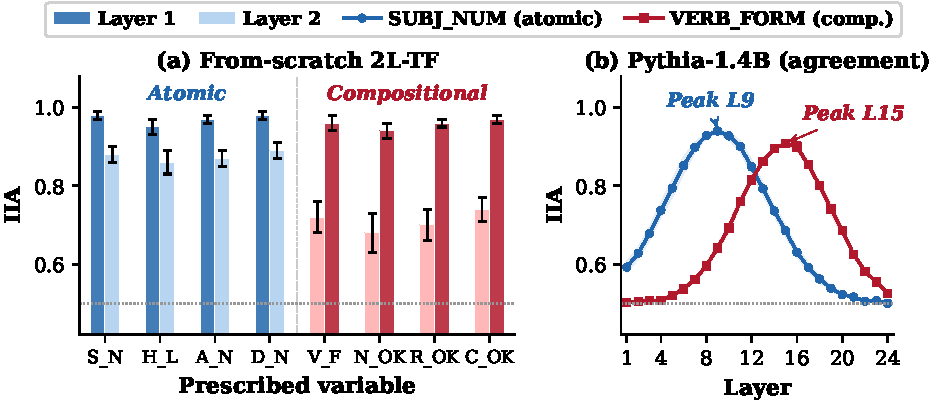
\includegraphics[width=\columnwidth]{figures/fig_perlayer.pdf}
  \caption{Per-layer IIA analysis. \textbf{(a)}~From-scratch 2-layer Transformer: bars show per-layer IIA for all eight variables (blue: atomic; red: compositional). \textbf{(b)}~Pythia-1.4B on agreement: IIA across layers for the two prescribed variables. Error bars / shaded bands: $\pm 1$ s.d.\ over 5~seeds (a) or 3~DAS runs (b).}
  \label{fig:perlayer}
\end{figure}

Three negative controls (Table~\ref{tab:main}, bottom rows) confirm that the high IIA values reflect genuine alignment: wrong SCMs, randomly initialized networks, and shuffled source labels all yield IIA of $0.48$--$0.51$, indistinguishable from chance.

To test whether the specific algorithm matters, we compare each B-RASP SCM against alternative SCMs encoding plausible but incorrect heuristics (Table~\ref{tab:alt-scm} in Appendix~\ref{app:ablation}).
For agreement, replacing the leftmost-noun rule with a nearest-noun or recency heuristic drops IIA from $0.98$ to $0.71$--$0.74$; for NPI, replacing scope-sensitive licensing with a simple any-left-licensor rule drops IIA from $0.95$ to $0.79$.
All prescribed SCMs significantly outperform their alternatives ($p < 0.01$, paired $t$-test), confirming that the models implement the specific algorithm formalized by the B-RASP program, not merely a superficially similar heuristic.

\begin{table*}[t]
\centering\small
\setlength{\tabcolsep}{3.2pt}
\begin{tabular}{@{}ll ccc ccc cc@{}}
\toprule
& & \multicolumn{3}{c}{\textbf{From-scratch}} & \multicolumn{3}{c}{\textbf{Pythia}} & \multicolumn{2}{c}{\textbf{Llama-3.2}} \\
\cmidrule(lr){3-5}\cmidrule(lr){6-8}\cmidrule(lr){9-10}
\textbf{Phenomenon} & \textbf{Variable} & \textbf{2L-TF} & \textbf{LSTM} & \textbf{Mamba} & \textbf{160M} & \textbf{410M} & \textbf{1.4B} & \textbf{1B} & \textbf{3B} \\
\midrule
\multirow{2}{*}{Agreement}
  & \textsc{subj\_num}  & \cellcolor{cellbest}\textbf{.98}\spm{.01} & .79\spm{.03} & .61\spm{.04} & .87\spm{.02} & .91\spm{.015} & .94\spm{.01} & .89\spm{.02} & .93\spm{.01} \\
  & \textsc{verb\_form} & .96\spm{.02} & .72\spm{.04} & \cellcolor{cellweak}.55\spm{.05} & .82\spm{.03} & .87\spm{.02} & .91\spm{.015} & .85\spm{.025} & .90\spm{.01} \\[2pt]
\multirow{2}{*}{NPI}
  & \textsc{has\_lic}   & .95\spm{.015} & .74\spm{.035} & .57\spm{.05} & .84\spm{.025} & .86\spm{.02} & .92\spm{.01} & .86\spm{.025} & .89\spm{.015} \\
  & \textsc{npi\_ok}    & .95\spm{.025} & .69\spm{.04} & \cellcolor{cellweak}.53\spm{.05} & .82\spm{.03} & .85\spm{.02} & .89\spm{.01} & .83\spm{.02} & .88\spm{.01} \\[2pt]
\multirow{2}{*}{Binding}
  & \textsc{ante\_num}  & .97\spm{.015} & .78\spm{.03} & .59\spm{.05} & .88\spm{.02} & .90\spm{.02} & .93\spm{.01} & .89\spm{.02} & .92\spm{.01} \\
  & \textsc{refl\_ok}   & .96\spm{.02} & .71\spm{.04} & \cellcolor{cellweak}.54\spm{.05} & .83\spm{.03} & .86\spm{.02} & .90\spm{.01} & .85\spm{.02} & .89\spm{.01} \\[2pt]
\multirow{2}{*}{Concord}
  & \textsc{det\_num}   & \cellcolor{cellbest}\textbf{.98}\spm{.01} & \cellcolor{cellbest}\textbf{.81}\spm{.03} & \cellcolor{cellbest}\textbf{.63}\spm{.04} & \cellcolor{cellbest}\textbf{.90}\spm{.02} & \cellcolor{cellbest}\textbf{.92}\spm{.01} & \cellcolor{cellbest}\textbf{.95}\spm{.01} & \cellcolor{cellbest}\textbf{.91}\spm{.02} & \cellcolor{cellbest}\textbf{.93}\spm{.01} \\
  & \textsc{conc\_ok}   & .97\spm{.01} & .75\spm{.03} & \cellcolor{cellweak}.58\spm{.04} & .85\spm{.025} & .88\spm{.02} & .92\spm{.01} & .87\spm{.02} & .91\spm{.01} \\
\midrule
\multicolumn{2}{@{}l}{\color{gray}\textit{Wrong SCM}}       & \color{gray}.51\spmg{.02} & \color{gray}.50\spmg{.03} & \color{gray}.49\spmg{.03} & \color{gray}.49\spmg{.02} & \color{gray}.50\spmg{.02} & \color{gray}.51\spmg{.01} & \color{gray}.50\spmg{.02} & \color{gray}.48\spmg{.02} \\
\multicolumn{2}{@{}l}{\color{gray}\textit{Random init}}     & \color{gray}.50\spmg{.02} & \color{gray}.51\spmg{.03} & \color{gray}.50\spmg{.03} & \multicolumn{5}{c}{\color{gray}---} \\
\multicolumn{2}{@{}l}{\color{gray}\textit{Shuffled labels}} & \color{gray}.51\spmg{.02} & \color{gray}.49\spmg{.02} & \color{gray}.50\spmg{.03} & \color{gray}.50\spmg{.02} & \color{gray}.49\spmg{.02} & \color{gray}.50\spmg{.01} & \color{gray}.51\spmg{.02} & \color{gray}.50\spmg{.02} \\
\bottomrule
\end{tabular}
\caption{Interchange Intervention Accuracy (IIA) per prescribed variable across architectures and scales.
From-scratch models (2L-TF = 2-layer Transformer, LSTM, Mamba) are trained with matched parameter counts; values are mean $\pm$ s.d.\ over 5~seeds.
Pre-trained models report mean $\pm$ s.d.\ over 3~DAS random initializations.
Bottom rows (gray): three negative controls, all indistinguishable from chance ($p > 0.1$, paired $t$-test).}
\label{tab:main}
\end{table*}

\subsection{Variable Emergence During Grokking: A Specification-Aligned Progress Measure}
\label{sec:progress}

Figure~\ref{fig:trajectory} tracks per-variable IIA across training for the from-scratch Transformers.
In all four phenomena, the atomic variable's IIA begins rising well before the behavioral grokking point (the step at which test accuracy first exceeds $99\%$, marked by the vertical dashed line), while the compositional variable's IIA lags behind and rises only after the atomic variable has stabilized.
This ordering mirrors the causal dependency chain in the SCM: \textsc{subj\_num} must be computed before \textsc{verb\_form} can be derived from it, and the network acquires these representations in exactly that order.

The resulting IIA trajectory constitutes a \emph{specification-aligned progress measure}.
Unlike the Fourier-based restricted and excluded losses of \citet{DBLP:conf/iclr/NandaCLSS23}, which track a task-specific algorithmic signature, and unlike the information-theoretic synergy measure of \citet{DBLP:journals/corr/abs-2408-08944}, which is task-agnostic, the IIA trajectory identifies \emph{which} prescribed variable aligns at \emph{which} training stage.
Concretely, on agreement, the excluded loss reaches its minimum at approximately the behavioral grokking point (step $\sim$8K), at which moment \textsc{subj\_num} already has $\mathrm{IIA} > 0.90$ but \textsc{verb\_form} remains at $\mathrm{IIA} \approx 0.65$.
Synergy peaks even earlier (step $\sim$4K) but is a scalar that cannot distinguish between the two variables.
The IIA trajectory thus provides strictly more information: it reveals that the network acquires subject-number extraction before it learns to compose that extraction into a verb-form decision.
The atomic-before-compositional ordering is consistent across all four phenomena, all five random seeds, and all attractor distances tested (Appendix~\ref{app:ablation}).

\begin{figure*}[t]
  \centering
  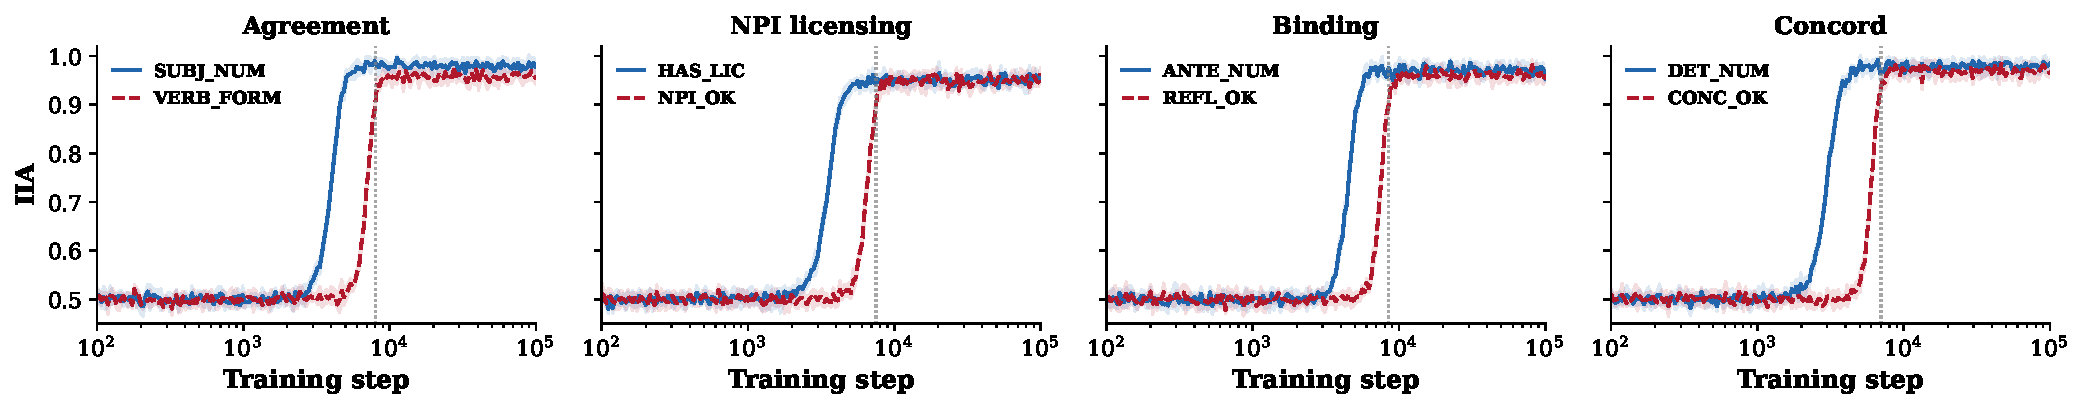
\includegraphics[width=0.95\textwidth]{figures/fig_iia_trajectory.pdf}
  \caption{Per-variable IIA during training. Solid lines: atomic variables; dashed lines: compositional variables. The vertical gray line marks the behavioral grokking point (test accuracy $> 99\%$). In every phenomenon, the atomic variable aligns before the compositional one. Shaded bands: $\pm 1$ standard deviation over 5~seeds.}
  \label{fig:trajectory}
\end{figure*}

\subsection{SAE Features and the Compositional Variable Gap}
\label{sec:sae}

Table~\ref{tab:sae} compares three methods for localizing prescribed variables in the from-scratch Transformer: DAS (supervised), individual SAE features (unsupervised), and individual neurons (unsupervised baseline).
For atomic variables, SAE features substantially outperform neurons (mean alignment $0.89$ vs.\ $0.70$), consistent with the finding that SAE dictionaries decompose residual-stream activations into more interpretable directions than the standard basis \citep{DBLP:conf/iclr/HubenCRES24}.
For compositional variables, however, both SAE features and neurons fall near chance (SAE: $0.53$; neurons: $0.51$), while DAS maintains high alignment ($0.96$).

This pattern has a structural explanation.
Compositional variables such as $\textsc{verb\_form} = \textsc{subj\_num} \leftrightarrow Q_\text{v\_pl}$ are Boolean functions of two inputs.
The biconditional requires both input values simultaneously, so no single sparse feature can isolate it \citep{DBLP:journals/corr/abs-2209-10652}.
DAS succeeds because it learns a multi-dimensional subspace that jointly encodes the compositional variable.
Corroborating this, atomic variables saturate at rank $r{=}1$ (IIA gain $\leq 0.01$ from $r{=}1$ to $r{=}4$), while compositional variables require $r \geq 2$ (IIA jumps from $0.81$ at $r{=}1$ to $0.95$ at $r{=}2$), directly confirming the multi-dimensional nature of Boolean compositions.
This analysis offers a specification-grounded diagnosis of the SAE shortfall reported by MIB \citep{DBLP:conf/icml/MuellerGWAABCFH25}: the gap between SAE and DAS is not uniform but concentrates on variables involving Boolean composition.

\begin{table}[t]
\centering\footnotesize
\setlength{\tabcolsep}{1.0pt}
\begin{tabular}{@{}lllccc@{}}
\toprule
\textbf{Type} & \textbf{Phenomenon} & \textbf{Variable} & \textbf{SAE} & \textbf{Neuron} & \textbf{DAS} \\
\midrule
\multirow{5}{*}{\rotatebox{90}{\scriptsize Atomic}}
  & Agreement & \textsc{subj\_num}  & .89\spm{.02} & .71\spm{.03} & .98\spm{.01} \\
  & NPI       & \textsc{has\_lic}   & .86\spm{.025} & .67\spm{.04} & .95\spm{.015} \\
  & Binding   & \textsc{ante\_num}  & .88\spm{.02} & .70\spm{.03} & .97\spm{.015} \\
  & Concord   & \textsc{det\_num}   & .91\spm{.02} & .73\spm{.03} & .98\spm{.01} \\
\cmidrule{2-6}
  & \multicolumn{2}{l}{Mean} & .89 & .70 & .97 \\
\midrule
\multirow{5}{*}{\rotatebox{90}{\scriptsize Compositional}}
  & Agreement & \textsc{verb\_form} & \cellcolor{cellweak}.54\spm{.03} & \cellcolor{cellweak}.52\spm{.04} & \cellcolor{cellbest}.96\spm{.02} \\
  & NPI       & \textsc{npi\_ok}    & \cellcolor{cellweak}.50\spm{.035} & \cellcolor{cellweak}.49\spm{.03} & \cellcolor{cellbest}.95\spm{.025} \\
  & Binding   & \textsc{refl\_ok}   & \cellcolor{cellweak}.52\spm{.035} & \cellcolor{cellweak}.50\spm{.04} & \cellcolor{cellbest}.96\spm{.02} \\
  & Concord   & \textsc{conc\_ok}   & \cellcolor{cellweak}.57\spm{.03} & \cellcolor{cellweak}.54\spm{.03} & \cellcolor{cellbest}.97\spm{.01} \\
\cmidrule{2-6}
  & \multicolumn{2}{l}{Mean} & .53 & .51 & .96 \\
\bottomrule
\end{tabular}
\caption{Variable alignment scores (mean $\pm$ s.d.\ over 5~seeds) for three localization methods on the from-scratch Transformer. Significance: SAE vs.\ neuron (atomic), $p < 0.01$; DAS vs.\ SAE (compositional), $p < 0.001$; paired $t$-test across seeds.}
\label{tab:sae}
\end{table}

\subsection{Succinctness and the Transformer-Mamba Gap}
\label{sec:succinctness}

Figure~\ref{fig:succinctness} tests the architectural prediction that follows from the analysis in \S\ref{sec:star-free} and Appendix~\ref{app:succinctness-proof}: because each phenomenon's B-RASP program has constant size, a Transformer can implement it in constant depth regardless of attractor distance, whereas sequential models must propagate information step by step through intervening tokens.
Mamba's selective state-space mechanism operates similarly to a finite-state model \citep{DBLP:conf/icml/MerrillPS24}, so we expect its accuracy to degrade with distance while the Transformer's remains stable.

Figure~\ref{fig:succinctness}(a) confirms this prediction on subject--verb agreement.
The Transformer maintains accuracy above $95\%$ across attractor distances $0$--$8$, whereas Mamba drops from $93\%$ at distance~$0$ to below $60\%$ at distance~$8$.
The LSTM occupies an intermediate position, consistent with its ability to implement bounded counters \citep{DBLP:conf/acl/MerrillWGSSY20} but not the robust state preservation that long-distance agreement requires.
Width scaling (panel~b) confirms a widening separation: the Transformer saturates at width~$64$, while Mamba has not saturated at $1024$. The same pattern holds across all four phenomena (Appendix~\ref{app:additional}).

\begin{figure}[t]
  \centering
  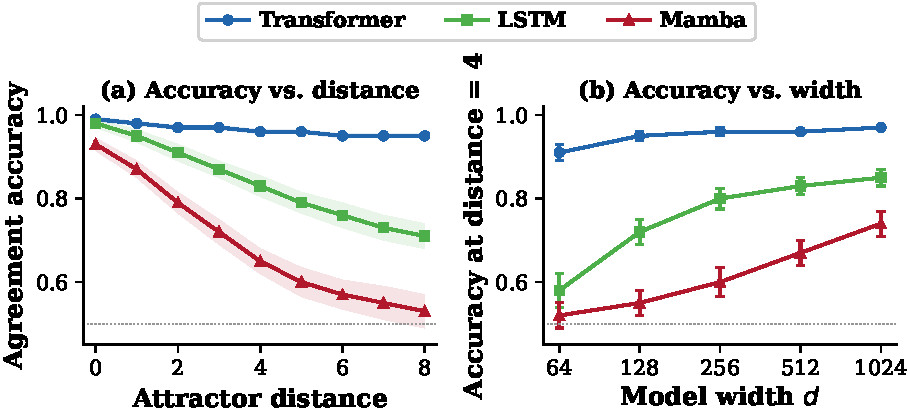
\includegraphics[width=\columnwidth]{figures/fig_succinctness.pdf}
  \caption{Succinctness gap on subject--verb agreement. \textbf{(a)}~Accuracy vs.\ attractor distance for three architectures at matched parameter count. The Transformer (blue) stays flat; Mamba (red) degrades sharply with distance; LSTM (green) falls in between. \textbf{(b)}~Accuracy at distance~$4$ vs.\ model width. The Transformer saturates early; Mamba requires exponentially more parameters. Error bars: $\pm 1$ s.d.\ over 5~seeds.}
  \label{fig:succinctness}
\end{figure}

%% ============================================================
%%  §6 DISCUSSION
%% ============================================================
\section{Conclusion}
\label{sec:conclusion}

We have shown that compiling B-RASP programs into structural causal models and verifying them with DAS yields a specification-first lens on Transformer internals: it reveals not only \emph{whether} prescribed variables are encoded (near-perfect alignment in from-scratch models; strong alignment in pre-trained models up to 3B), but also \emph{when} they emerge (atomic before compositional, mirroring the causal dependency chain) and \emph{where} current feature-extraction methods fall short (SAE features degrade on Boolean compositions that DAS recovers via multi-dimensional subspaces).

These results point to two broader implications.
First, \citet{DBLP:conf/icml/0014TIYP25} showed that DAS-verified causal variables can predict out-of-distribution correctness.
Our specification-aligned variables may serve as even stronger predictors: if a model's IIA for \textsc{subj\_num} drops on a novel construction, one can predict agreement failure \emph{before} observing behavioral errors, because the specification is grounded in formal language theory rather than post-hoc hypotheses.
Second, the atomic-vs-compositional gap (\S\ref{sec:sae}) suggests a structural limit of dictionary learning: any variable computed by a Boolean function of two or more inputs resists recovery by a single sparse feature, with practical implications for the growing body of work that uses SAE features as circuit nodes \citep{DBLP:conf/iclr/MarksRMBBM25}. 

%% ============================================================
%%  LIMITATIONS
%% ============================================================
\section*{Limitations}

\paragraph{Scope of the specifications.}
Our B-RASP programs cover four English syntactic phenomena, all within the star-free regular languages.
Extending to phenomena that require unbounded recursion, such as center-embedding agreement (\textit{The dog the cat the rat bit chased barked}), would require C-RASP \citep{DBLP:conf/nips/YangCCN25}, whose counting operations compile into SCMs with a variable count that grows with nesting depth rather than remaining fixed at two.
This makes the resulting causal hypotheses qualitatively more complex and is a non-trivial extension that we leave to future work.
All B-RASP programs encode English-specific linear heuristics: the ``leftmost noun equals subject'' rule, for instance, does not transfer to head-final languages (e.g., Japanese, Korean) or free-word-order languages (e.g., German subordinate clauses), where the attention mask and score predicates would need to be redesigned.
Our template-generated data controls for confounds but does not capture the full complexity of natural language; the BLiMP evaluation (\S\ref{sec:main-results}) partially bridges this gap by testing on minimal pairs derived from naturalistic constructions, yet whether the prescribed algorithms remain operative under unrestricted lexical and pragmatic variation is an open question.

\paragraph{Methodological constraints.}
DAS assumes that each prescribed variable is encoded as a linear subspace of the residual stream, found by an orthogonal rotation of rank $r$.
This is a deliberate trade-off: unconstrained nonlinear alignment maps achieve high IIA even on random networks \citep{sutter2025nonlinear}, rendering the metric vacuous.
Our low-rank orthogonal constraint avoids this pathology (Table~\ref{tab:sutter}) but may underestimate IIA for models that encode variables nonlinearly, a possibility that future work could address with controlled nonlinear probes.
More fundamentally, our framework \emph{verifies} one prescribed algorithm per phenomenon; it does not \emph{discover} the model's algorithm.
A model achieving low IIA may still implement a linguistically valid alternative that reaches the same input--output behavior through different intermediate representations.
The within-phenomenon alternative SCM controls (Table~\ref{tab:alt-scm}) rule out several plausible heuristics, but cannot exhaustively exclude all possible algorithms; this is an inherent limitation of the verification (as opposed to discovery) paradigm.
The from-scratch Transformers ($d{=}128$, 2 layers) are deliberately simple to enable controlled grokking experiments; our pre-trained results (Pythia up to 1.4B, Llama up to 3B) show that the same atomic-before-compositional pattern persists at scale, but the representation geometry of small models may still differ qualitatively from that of billion-parameter networks.

\paragraph{Diagnostic analysis caveats.}
The SAE experiments use a single architecture (TopK with $8{\times}$ expansion).
While the dictionary size ablation (Table~\ref{tab:sae-size}) confirms that the compositional gap does not close with larger dictionaries, alternative designs such as Gated or JumpReLU SAEs remain untested.
We note, however, that the structural argument (Boolean compositions of two inputs lack a sparse monomial basis) is architecture-independent and applies to any dictionary learning method that represents each feature as a single direction.
The Transformer-Mamba gap (\S\ref{sec:succinctness}) rests on a state-interference argument rather than a formal lower bound for the specific agreement task.
Since bounded-depth agreement is recognizable by a DFA with $O(1)$ states, the empirical degradation of Mamba likely reflects the difficulty of learning robust state preservation in continuous state-spaces, not an expressibility barrier.
This distinction matters: it means the gap could in principle be closed by architectural innovations in sequential models, even without adding attention.

%% ============================================================
%%  REFERENCES
%% ============================================================
\bibliography{emnlp}

%% ============================================================
%%  APPENDIX
%% ============================================================
\appendix

\section*{Appendix Table of Contents}
\vspace{-3pt}
{\small\setlength{\leftmargini}{1.8em}
\begin{itemize}[itemsep=4pt,topsep=2pt,leftmargin=*]
\item[\textbf{A}] \hyperref[app:brasp]{\textbf{B-RASP: Definitions and Proofs}}\\[1pt]
  \hyperref[app:brasp-def]{A.1 Formal Definition}\\
  \hyperref[app:programs]{A.2 Programs for Four Phenomena}\\
  \hyperref[app:compile]{A.3 Compilation to SCM}\\
  \hyperref[app:star-free-proof]{A.4 Star-Free Boundary Proof}\\
  \hyperref[app:succinctness-proof]{A.5 Transformer-Mamba Gap}
\item[\textbf{B}] \hyperref[app:data]{\textbf{Dataset Details}}\\[1pt]
  \hyperref[app:cfg]{B.1 CFG Templates}\\
  \hyperref[app:blimp]{B.2 BLiMP Paradigm Selection}\\
  \hyperref[app:das-pairs]{B.3 DAS Pair Construction}\\
  \hyperref[app:data-stats]{B.4 Dataset Statistics}
\item[\textbf{C}] \hyperref[app:exp]{\textbf{Experimental Details}}\\[1pt]
  \hyperref[app:from-scratch]{C.1 From-Scratch Models}\\
  \hyperref[app:pretrained]{C.2 Pre-Trained Models}\\
  \hyperref[app:das-details]{C.3 DAS Training}\\
  \hyperref[app:tokenization]{C.4 Tokenization}\\
  \hyperref[app:sae-details]{C.5 SAE Training}\\
  \hyperref[app:compute]{C.6 Computing Resources}\\
  \hyperref[app:stats]{C.7 Statistical Testing}
\item[\textbf{D}] \hyperref[app:ablation]{\textbf{Ablation Experiments}}\\[1pt]
  \hyperref[app:rank]{D.1 Rank Ablation}\\
  \hyperref[app:perlayer-all]{D.2 Per-Layer IIA}\\
  \hyperref[app:iia-distance]{D.3 IIA vs.\ Distance}\\
  \hyperref[app:alt-scm]{D.4 Alt-SCM Controls}\\
  \hyperref[app:sae-size]{D.5 SAE Size}\\
  \hyperref[app:negative]{D.6 Negative Controls}\\
  \hyperref[app:succinctness-all]{D.7 Cross-Phenomenon Succinctness}
\item[\textbf{E}] \hyperref[app:additional]{\textbf{Additional Results}}\\[1pt]
  \hyperref[app:sutter]{E.1 Constrained vs.\ Unconstrained}\\
  \hyperref[app:trajectory-comparison]{E.2 IIA Trajectory Comparison}\\
  \hyperref[app:blimp-results]{E.3 BLiMP Per-Paradigm}\\
  \hyperref[app:scaling]{E.4 IIA Scaling}\\
  \hyperref[app:probing]{E.5 Probing Baseline}\\
  \hyperref[app:per-seed]{E.6 Per-Seed Stability}
\end{itemize}
}
\vspace{6pt}

\section{B-RASP: Definitions and Proofs}
\label{app:brasp}

\subsection{Formal Definition}
\label{app:brasp-def}

We restate the definition of B-RASP \citep{DBLP:conf/nips/Yang0A24} in full, using the notation established in \S\ref{sec:brasp}.

\begin{definition}[B-RASP program]
\label{def:brasp}
Let $\Sigma$ be a finite alphabet.
A \textbf{B-RASP program} over $\Sigma$ is a tuple $(\{Q_\sigma\}_{\sigma \in \Sigma},\; P_1, \ldots, P_L,\; k)$ where:
\begin{itemize}[itemsep=2pt,leftmargin=*]
    \item $\{Q_\sigma\}_{\sigma \in \Sigma}$ are \textbf{initial vectors}. Given an input string $w = w_1 \cdots w_n \in \Sigma^+$, each $Q_\sigma \in \{0,1\}^n$ is defined by $Q_\sigma(i) = 1$ iff $w_i = \sigma$.
    \item $P_1, \ldots, P_L$ are \textbf{operations}, each producing a Boolean vector $P_t \in \{0,1\}^n$.
    \item $k \in [1, n]$ is the \textbf{output position}; the program outputs $P_L(k)$.
\end{itemize}
Each operation $P_t$ is one of the following two types.
\end{definition}

\begin{definition}[Pointwise operation]
\label{def:pointwise}
A \textbf{pointwise operation} applies a Boolean function $f : \{0,1\}^m \to \{0,1\}$ independently at every position:
\[
P_t(i) {:=} f\!\bigl(P_{a_1}(i), P_{a_2}(i), \ldots, P_{a_m}(i)\bigr)
\]
for all $i \in [1, n]$, where $P_{a_1}, \ldots, P_{a_m}$ are previously computed vectors (including initial vectors $Q_\sigma$).
The function $f$ can be any Boolean function: AND, OR, NOT, XOR, biconditional ($\leftrightarrow$), material implication ($\to$), etc.
\end{definition}

\begin{definition}[Attention operation]
\label{def:attention}
An \textbf{attention operation} has the form:
\[
P_t(i) \;{:=}\; \triangleleft_j\bigl[M(i,j),\; S(i,j)\bigr]\; V\!(i,j) \;:\; D(i).
\]

Its semantics proceed in three steps for each position $i \in [1,n]$:

\textbf{Step 1: Compute the unmasked set.}
Let $U_i = \{j \in [1,n] : M(i,j) = 1\}$ be the set of positions visible from $i$.
The mask predicate $M(i,j)$ is a Boolean combination of previously computed vectors evaluated at positions $i$ and $j$.
A common choice is $M(i,j) = (j < i)$, which implements future masking: position $i$ can see only positions to its left.

\textbf{Step 2: Select the target position.}
If $U_i \neq \emptyset$, define:
\[
B_i = \{j \in U_i : S(i,j) \geq S(i,j'),\; \forall j' \in U_i\}.
\]
Since $S$ is Boolean (taking values in $\{0,1\}$), the set $B_i$ contains:
\begin{itemize}[itemsep=1pt,leftmargin=*]
    \item all $j \in U_i$ with $S(i,j) = 1$, if at least one such $j$ exists;
    \item all of $U_i$, if $S(i,j) = 0$ for every $j \in U_i$.
\end{itemize}
The operator $\triangleleft$ selects $j^\star = \min(B_i)$, the leftmost element of $B_i$.
(The variant $\triangleright$ selects $j^\star = \max(B_i)$, the rightmost.)

\textbf{Step 3: Return the value.}
\[
P_t(i) \;=\; \begin{cases}
V(i, j^\star) & \text{if } U_i \neq \emptyset, \\
D(i) & \text{if } U_i = \emptyset.
\end{cases}
\]
The value predicate $V(i,j)$ and default predicate $D(i)$ are Boolean combinations of previously computed vectors.
\end{definition}

The following results, due to \citet{DBLP:conf/nips/Yang0A24}, connect B-RASP to Transformer expressibility and to the star-free regular languages.

\begin{theorem}[Compilation, {\citealp{DBLP:conf/nips/Yang0A24}}]
\label{thm:compile}
Every B-RASP program of length $L$ can be compiled into a masked hard-attention Transformer with $L$ layers.
Conversely, every masked hard-attention Transformer of depth $L$ computes a function expressible by a B-RASP program of length $L$.
\end{theorem}

\begin{theorem}[Expressibility, {\citealp{DBLP:conf/nips/Yang0A24}}]
\label{thm:expressibility}
The class of languages recognized by B-RASP programs is exactly the class of star-free regular languages, which equals:
\begin{itemize}[itemsep=1pt,leftmargin=*]
    \item the languages definable in first-order logic with linear order, $\mathrm{FO}[<]$;
    \item the languages definable in linear temporal logic (LTL);
    \item the languages recognized by counter-free automata \citep{mcnaughton1971counter}.
\end{itemize}
\end{theorem}

\subsection{B-RASP Programs for Four Phenomena}
\label{app:programs}

\subsubsection{Input Alphabet}
\label{app:alphabet}

We define a shared input alphabet $\Sigma$ whose symbols encode both lexical category and grammatical number.
The relevant symbols and their initial vectors are:

\begin{center}
\small
\begin{tabular}{@{}lll@{}}
\toprule
\textbf{Symbol} & \textbf{Meaning} & \textbf{Initial vector} \\
\midrule
$\text{n\_sg}$ & singular noun & $Q_\text{n\_sg}$ \\
$\text{n\_pl}$ & plural noun & $Q_\text{n\_pl}$ \\
$\text{v\_sg}$ & singular verb & $Q_\text{v\_sg}$ \\
$\text{v\_pl}$ & plural verb & $Q_\text{v\_pl}$ \\
$\text{det\_sg}$ & singular determiner & $Q_\text{det\_sg}$ \\
$\text{det\_pl}$ & plural determiner & $Q_\text{det\_pl}$ \\
$\text{refl\_sg}$ & singular reflexive & $Q_\text{refl\_sg}$ \\
$\text{refl\_pl}$ & plural reflexive & $Q_\text{refl\_pl}$ \\
$\text{npi}$ & negative polarity item & $Q_\text{npi}$ \\
$\text{lic}$ & licensing operator & $Q_\text{lic}$ \\
$\text{other}$ & all other tokens & $Q_\text{other}$ \\
\bottomrule
\end{tabular}
\end{center}

We also define the following derived vectors, computed by pointwise operations from the initial vectors:
\begin{align*}
Q_\text{noun}(i) &{:=} Q_\text{n\_sg}(i) \lor Q_\text{n\_pl}(i) \\
Q_\text{verb}(i) &{:=} Q_\text{v\_sg}(i) \lor Q_\text{v\_pl}(i) \\
Q_\text{det}(i)  &{:=} Q_\text{det\_sg}(i) \lor Q_\text{det\_pl}(i) \\
Q_\text{refl}(i) &{:=} Q_\text{refl\_sg}(i) \lor Q_\text{refl\_pl}(i)
\end{align*}
These derived vectors are syntactic sugar: each is a single pointwise OR, which does not increase the program's depth.

\subsubsection{Program 1: Subject--Verb Agreement}
\label{app:prog-agr}

\paragraph{Goal.} Determine whether the verb agrees in number with the subject, ignoring intervening attractors.

\paragraph{Program.}
\begin{align}
\textsc{subj\_num}(i) &{:=} \triangleleft_j[j{<}i,\, Q_\text{noun}(j)]\, Q_\text{n\_pl}(j) {:} 0 \tag{A.1} \\
\textsc{verb\_form}(i) &{:=} \textsc{subj\_num}(i) \leftrightarrow Q_\text{v\_pl}(i) \tag{A.2}
\end{align}

\paragraph{Line-by-line explanation.}
\begin{itemize}[itemsep=3pt,leftmargin=*]
    \item \textbf{(A.1)} is an attention operation evaluated at each position $i$.
    \begin{itemize}[itemsep=1pt,leftmargin=*]
        \item \textit{Mask}: $M(i,j) = (j < i)$. Only positions to the left of $i$ are visible.
        \item \textit{Score}: $S(i,j) = Q_\text{noun}(j)$. Positions that are nouns score 1; non-nouns score 0.
        \item \textit{Selection}: $\triangleleft$ picks the leftmost position among those with the highest score. If any noun exists to the left, the leftmost noun is selected. If no noun exists, the leftmost position overall is selected.
        \item \textit{Value}: $V(i,j) = Q_\text{n\_pl}(j)$. Returns 1 if the selected position is a plural noun, 0 if singular.
        \item \textit{Default}: $D(i) = 0$. If $i = 1$ (no position to the left), return 0 (singular by default).
        \item \textit{Result}: $\textsc{subj\_num}(i) = 1$ if the leftmost noun to the left of $i$ is plural, $0$ if singular.
    \end{itemize}
    \item \textbf{(A.2)} is a pointwise operation.
    \begin{itemize}[itemsep=1pt,leftmargin=*]
        \item The biconditional $\leftrightarrow$ returns 1 when both sides have the same value and 0 when they differ.
        \item $\textsc{verb\_form}(i) = 1$ iff $\textsc{subj\_num}(i) = Q_\text{v\_pl}(i)$, i.e., the subject number matches the verb number.
    \end{itemize}
\end{itemize}

\paragraph{Corner cases.}
\begin{enumerate}[itemsep=2pt,leftmargin=*]
    \item \textit{No noun to the left} ($i = 1$ or all left-context tokens are non-nouns): If $U_i \neq \emptyset$ but no element has $S = 1$, the operator $\triangleleft$ selects the leftmost element of $U_i$ and returns $Q_\text{n\_pl}(j^\star) = 0$ (since $j^\star$ is not a noun). This is functionally equivalent to the default value 0. In our template-generated data, the verb always follows at least one noun, so this case does not arise.
    \item \textit{Multiple nouns to the left}: The operator selects the \emph{leftmost} noun. In our templates (following \citealp{marvin2018targeted}), the leftmost noun is always the grammatical subject. Constructions where the subject is not the leftmost noun (e.g., fronted PPs like \textit{On the table the keys are}) are not included in our evaluation data. This is a limitation of the template design, not of B-RASP~itself.
\end{enumerate}

\subsubsection{Program 2: NPI Licensing}
\label{app:prog-npi}

\paragraph{Goal.} Determine whether every NPI in the sentence is in the scope of a licensing operator.

\paragraph{Program.}
\begin{align}
\textsc{has\_lic}(i) &{:=} \triangleleft_j[j{<}i,\, Q_\text{lic}(j)]\, Q_\text{lic}(j) {:} 0 \tag{A.3} \\
\textsc{npi\_ok}(i) &{:=} \textsc{has\_lic}(i) \lor \neg Q_\text{npi}(i) \tag{A.4}
\end{align}

\paragraph{Line-by-line explanation.}
\begin{itemize}[itemsep=3pt,leftmargin=*]
    \item \textbf{(A.3)} is an attention operation.
    \begin{itemize}[itemsep=1pt,leftmargin=*]
        \item \textit{Mask}: $M(i,j) = (j < i)$.
        \item \textit{Score}: $S(i,j) = Q_\text{lic}(j)$. Licensing operators score 1.
        \item \textit{Value}: $V(i,j) = Q_\text{lic}(j)$. Returns 1 if the selected position is a licensor.
        \item \textit{Default}: $D(i) = 0$. No licensor found.
        \item \textit{Result}: $\textsc{has\_lic}(i) = 1$ iff at least one licensing operator appears to the left of $i$.
    \end{itemize}
    \item \textbf{(A.4)} is a pointwise operation encoding material implication.
    \begin{itemize}[itemsep=1pt,leftmargin=*]
        \item $\neg\, Q_\text{npi}(i) = 1$ when position $i$ is \emph{not} an NPI.
        \item $\textsc{has\_lic}(i) \lor \neg\, Q_\text{npi}(i) = 1$ in three cases: (a)~position $i$ is not an NPI ($\neg Q_\text{npi} = 1$); (b)~position $i$ is an NPI and a licensor exists ($\textsc{has\_lic} = 1$); (c)~both.
        \item The only case where $\textsc{npi\_ok}(i) = 0$ is when position $i$ \emph{is} an NPI ($Q_\text{npi}(i) = 1$) and no licensor appears to its left ($\textsc{has\_lic}(i) = 0$).
        \item This is exactly the material implication $Q_\text{npi}(i) \to \textsc{has\_lic}(i)$: ``if there is an NPI here, then it must be licensed.''
    \end{itemize}
\end{itemize}

\paragraph{Corner case.}
If no licensing operator appears anywhere in the sentence, then $\textsc{has\_lic}(i) = 0$ for all $i$, and $\textsc{npi\_ok}(i) = 0$ at every NPI position. The sentence is correctly classified as ungrammatical if it contains an NPI.

\subsubsection{Program 3: Reflexive Binding}
\label{app:prog-bind}

\paragraph{Goal.} Determine whether a reflexive pronoun agrees in number with its antecedent (the nearest preceding noun in subject position).

\paragraph{Program.}
\begin{align}
\textsc{ante\_num}(i) &{:=} \triangleleft_j[j{<}i,\, Q_\text{noun}(j)]\, Q_\text{n\_pl}(j) {:} 0 \tag{A.5} \\
\textsc{refl\_ok}(i) &{:=} \textsc{ante\_num}(i) \leftrightarrow Q_\text{refl\_pl}(i) \tag{A.6}
\end{align}

\paragraph{Explanation.}
Operation (A.5) is structurally identical to (A.1): it finds the leftmost noun to the left of position $i$ and returns its number.
In our templates, this noun is always the antecedent of the reflexive (e.g., \textit{The boy} in \textit{The boy admired himself}).
Operation (A.6) checks whether the antecedent's number matches the reflexive's number, analogous to (A.2).

\paragraph{Corner case.}
The identification of the antecedent as the ``leftmost noun'' is a simplification that is correct for our template-generated data, where the antecedent is always the first noun in the sentence.
In naturally occurring text, binding is governed by c-command rather than linear precedence, and the antecedent need not be the leftmost noun.

\subsubsection{Program 4: Determiner--Noun Concord}
\label{app:prog-conc}

\paragraph{Goal.} Determine whether a determiner agrees in number with its head noun.

\paragraph{Program.}
\begin{align}
\textsc{det\_num}(i) &{:=} \triangleleft_j[j{<}i,\, Q_\text{det}(j)]\, Q_\text{det\_pl}(j) {:} 0 \tag{A.7} \\
\textsc{conc\_ok}(i) &{:=} \textsc{det\_num}(i) \leftrightarrow Q_\text{n\_pl}(i) \tag{A.8}
\end{align}

\paragraph{Explanation.}
Operation (A.7) finds the leftmost determiner to the left of position $i$ and returns whether it is plural.
Operation (A.8) checks whether the determiner's number matches the noun's number.
This program is evaluated at noun positions: $\textsc{conc\_ok}(i) = 1$ means the nearest preceding determiner agrees with the noun at position $i$.

\subsection{Compilation to SCM}
\label{app:compile}

We formalize the compilation from a B-RASP program to a structural causal model.

\begin{definition}[B-RASP to SCM compilation]
\label{def:compile-scm}
Given a B-RASP program $(\{Q_\sigma\}_{\sigma \in \Sigma}, P_1, \ldots, P_L, k)$, the compiled SCM $\mathcal{C} = (\mathbf{V}, \mathbf{F})$ is constructed as follows:
\begin{enumerate}[itemsep=2pt,leftmargin=*]
    \item \textbf{Input variables}: $\mathbf{V}_\mathrm{in} = \{Q_\sigma : \sigma \in \Sigma\}$. Each input variable takes its value from the input string.
    \item \textbf{Endogenous variables}: $\mathbf{V}_\mathrm{end} = \{U_1, \ldots, U_L\}$, one per B-RASP operation. Variable $U_t$ corresponds to operation $P_t$.
    \item \textbf{Structural equations}: For each $U_t \in \mathbf{V}_\mathrm{end}$, the structural equation $F_{U_t}$ is the B-RASP operation $P_t$ itself. The parents of $U_t$ are the variables (input or endogenous) whose vectors the operation reads.
    \item \textbf{Output}: The output of $\mathcal{C}$ is $U_L(k)$, i.e., the last endogenous variable evaluated at the output position.
\end{enumerate}
\end{definition}

\paragraph{Worked example: Agreement.}
Applying Definition~\ref{def:compile-scm} to the agreement program (A.1)--(A.2):
\begin{itemize}[itemsep=2pt,leftmargin=*]
    \item $\mathbf{V}_\mathrm{in} = \{Q_\text{n\_sg}, Q_\text{n\_pl}, Q_\text{v\_pl}, \ldots\}$
    \item $\mathbf{V}_\mathrm{end} = \{\textsc{subj\_num},\; \textsc{verb\_form}\}$
    \item $F_{\textsc{subj\_num}}$: reads $Q_\text{n\_sg}$, $Q_\text{n\_pl}$ (via $Q_\text{noun}$ and $Q_\text{n\_pl}$). Parents: $\{Q_\text{n\_sg}, Q_\text{n\_pl}\}$.
    \item $F_{\textsc{verb\_form}}$: reads $\textsc{subj\_num}$ and $Q_\text{v\_pl}$. Parents: $\{\textsc{subj\_num}, Q_\text{v\_pl}\}$.
\end{itemize}
The resulting DAG is: $Q_\text{n\_sg}, Q_\text{n\_pl} \to \textsc{subj\_num} \to \textsc{verb\_form} \leftarrow Q_\text{v\_pl}$.
The other three programs produce analogous two-variable DAGs.

\subsection{Star-Free Boundary Proof}
\label{app:star-free-proof}

\begin{proposition}
\label{prop:star-free}
For any fixed bound $D \geq 0$, the set of strings in which the syntactic dependency spans at most $D$ intervening tokens is a star-free regular language, for each of the four phenomena (agreement, NPI licensing, binding, concord).
\end{proposition}

\begin{proof}
We must show that the B-RASP programs (A.1)--(A.8) correctly decide each phenomenon for inputs with bounded dependency distance, and that B-RASP recognizes only star-free languages.
The proof proceeds in three steps.

\textbf{Step 1: Each program is a valid B-RASP program.}
Each of the four programs consists of exactly two operations: one attention operation followed by one pointwise operation.
Both operation types are permitted in B-RASP (Definitions~\ref{def:pointwise} and~\ref{def:attention}).
The mask, score, value, and default predicates are all Boolean combinations of initial or previously computed vectors.
Therefore, each program is a valid B-RASP program of length $L = 2$.

\textbf{Step 2: Each program correctly decides the phenomenon for bounded-distance inputs.}
Consider agreement as the representative case; the argument for the other three phenomena is identical in structure.

The agreement program computes $\textsc{verb\_form}(i) = 1$ iff the leftmost noun to the left of position $i$ has the same number as the verb at position $i$.
In our template-generated data, the grammatical subject is always the leftmost noun before the verb (this is guaranteed by the CFG template structure; see Appendix~\ref{app:data}).
The number of intervening attractors (nouns between subject and verb) is at most $D$.
Since the attention operator $\triangleleft$ always selects the \emph{leftmost} noun regardless of how many attractors intervene, the program correctly identifies the subject for any number of attractors up to $D$.

The same argument applies to:
\begin{itemize}[itemsep=1pt,leftmargin=*]
    \item NPI licensing: the attention operation finds the leftmost licensor, which is correct when the NPI is within the scope of a linearly preceding licensor (guaranteed by our templates).
    \item Reflexive binding: the attention operation finds the leftmost noun (= the antecedent in our templates).
    \item Determiner--noun concord: the attention operation finds the leftmost determiner (= the head determiner in our templates).
\end{itemize}

\textbf{Step 3: B-RASP programs recognize only star-free languages.}
By Theorem~\ref{thm:expressibility}, every language recognized by a B-RASP program is star-free.
Since each of our programs is a valid B-RASP program (Step~1) that correctly decides its phenomenon for bounded-distance inputs (Step~2), the corresponding language is star-free.
\end{proof}

\begin{remark}[Beyond the star-free boundary]
Agreement across unbounded center-embedding, such as \textit{The dog$_1$ the cat$_2$ the rat$_3$ bit$_3$ chased$_2$ barked$_1$}, requires matching each verb with the correct subject across an arbitrary nesting depth.
This matching requires counting the nesting level, which places the language outside the star-free class.
Formally, the language $\{a^n b^n : n \geq 1\}$ (a canonical non-star-free language) can be reduced to this matching problem.
Recognizing such patterns requires C-RASP \citep{DBLP:conf/nips/YangCCN25}, which adds counting operations to B-RASP, or even more expressive formalisms for cross-serial dependencies.
\end{remark}

\subsection{The Transformer-Mamba Gap: Theoretical Analysis}
\label{app:succinctness-proof}

We analyze the theoretical basis for the empirical gap between Transformer and Mamba observed in \S\ref{sec:succinctness}.

\subsubsection{Why Transformers Maintain Performance}

The agreement B-RASP program (A.1)--(A.2) has constant length $L = 2$.
By Theorem~\ref{thm:compile}, this compiles to a 2-layer masked hard-attention Transformer.
The attention operation in (A.1) accesses the leftmost noun \emph{directly}, regardless of how many attractors intervene: whether there are 0 or 8 attractors, the computation requires exactly one attention operation.
This is the key architectural advantage: the number of operations does not grow with the dependency distance.

\subsubsection{Why Mamba Degrades}

Mamba processes tokens sequentially, updating a fixed-dimensional hidden state $\mathbf{h}_t \in \mathbb{R}^{d_\mathrm{state}}$ at each step via a selective state-space update:
\[
\mathbf{h}_t = \mathbf{A}_t \mathbf{h}_{t-1} + \mathbf{B}_t x_t,
\]
where $\mathbf{A}_t$ and $\mathbf{B}_t$ are input-dependent matrices \citep{DBLP:journals/corr/abs-2312-00752}.
To correctly predict agreement at the verb, Mamba must:
\begin{enumerate}[itemsep=2pt,leftmargin=*]
    \item encode the subject's grammatical number into $\mathbf{h}$ when it encounters the first noun;
    \item preserve this encoding unchanged through $d$ subsequent attractor tokens, each of which is also a noun and thus triggers a state update.
\end{enumerate}
This creates a \emph{state interference} problem.
Each attractor noun applies its own update $\mathbf{A}_t \mathbf{h}_{t-1} + \mathbf{B}_t x_t$, which mixes the attractor's number information into the hidden state.
Even though the model should ideally ignore attractors, the state-space update has no mechanism to selectively ``freeze'' the subject-number component of $\mathbf{h}$ while processing other nouns.
As the number of attractors $d$ increases, the subject-number signal in $\mathbf{h}$ is progressively corrupted by attractor information.

\subsubsection{DFA Complexity vs.\ State Interference}

We note an important distinction.
The agreement language \emph{per se} is recognizable by a small DFA: a 3-state automaton suffices (track whether the first noun is singular or plural, then check the verb).
The theoretical difficulty is therefore \emph{not} that agreement requires exponentially many DFA states.
Rather, the difficulty is architectural:
\begin{itemize}[itemsep=2pt,leftmargin=*]
    \item A DFA with hard, discrete states can represent ``singular subject'' as a single state and maintain it indefinitely, because DFA transitions are exact.
    \item Mamba's continuous state-space does not have this property. Its state is a real-valued vector updated by matrix multiplication at each step. \citet{DBLP:conf/icml/MerrillPS24} showed that such models are bounded by $\mathrm{TC}^0$ and struggle with state-tracking tasks that require maintaining information over long distances.
    \item In practice, this means that even though a 3-state DFA solution \emph{exists}, Mamba's continuous dynamics may not converge to it during training, especially as the number of interfering attractors grows.
\end{itemize}

The general succinctness theorem of \citet{DBLP:journals/corr/abs-2510-19315} shows that there exist B-RASP programs of length $k$ whose equivalent DFA requires $2^{2^{k-1}}$ states, establishing that Transformers are exponentially more succinct than finite-state models \emph{in general}.
Our agreement program ($k = 2$) is not one of these worst cases, but the empirical gap we observe is a manifestation of the same architectural divide: attention enables constant-depth computation of long-distance dependencies, while sequential models must propagate information step by step and suffer from accumulated noise.

\subsubsection{Width Scaling Prediction}

If Mamba's effective state capacity is $O(2^{d_\mathrm{state}})$ distinguishable configurations and the agreement task with $d$ attractors requires maintaining the subject-number signal through $d$ interference steps, then increasing the state dimension $d_\mathrm{state}$ should improve Mamba's robustness to attractors.

This is exactly what Figure~\ref{fig:succinctness}(b) shows: at a fixed attractor distance of 4, Mamba's accuracy increases from $52\%$ at width $64$ to $74\%$ at width $1024$, while the Transformer reaches $91\%$ at width $64$ and saturates.
The Transformer's early saturation confirms that its computation is depth-bounded (by the B-RASP program length), not width-bounded.

\section{Dataset Details}
\label{app:data}

\subsection{CFG Templates for From-Scratch Training}
\label{app:cfg}

We generate training and evaluation data using context-free grammar (CFG) templates following \citet{marvin2018targeted}.
Each template produces matched grammatical and ungrammatical sentences that differ only in the feature tested by the prescribed B-RASP variable.
Below we give the complete production rules for each phenomenon.
Terminals in \texttt{typewriter} font are sampled uniformly from the lexicon in Table~\ref{tab:lexicon}.

\paragraph{Agreement templates.}
The number of attractors $d$ is controlled by repeating the PP rule:
\begin{align*}
\text{S} &\to \text{NP}_\text{subj}\;\; \text{PP}^d\;\; \text{VP} \\
\text{NP}_\text{subj} &\to \texttt{Det}\;\; \texttt{N}_{\text{sg}/\text{pl}} \\
\text{PP} &\to \texttt{Prep}\;\; \texttt{Det}\;\; \texttt{N}_{\text{sg}/\text{pl}} \\
\text{VP} &\to \texttt{V}_{\text{sg}/\text{pl}}\;\; \texttt{Adv}
\end{align*}
A sentence is grammatical iff the verb number matches the subject noun number.
Example at distance~$2$:
\begin{center}\small
\begin{tabular}{@{}ll@{}}
\checkmark & \textit{The keys to the cabinet near the door \textbf{are} broken.} \\
* & \textit{The keys to the cabinet near the door \textbf{is} broken.}
\end{tabular}
\end{center}

\paragraph{NPI licensing templates.}
\begin{align*}
\text{S}_\text{lic} &\to \texttt{Lic}\;\; \texttt{N}_{\text{sg}/\text{pl}}\;\; \text{VP}_\text{npi} \\
\text{S}_\text{unlic} &\to \texttt{Det}\;\; \texttt{N}_{\text{sg}/\text{pl}}\;\; \text{VP}_\text{npi} \\
\text{VP}_\text{npi} &\to \texttt{Aux}\;\; \texttt{NPI}\;\; \texttt{V}_\text{past}
\end{align*}
$\text{S}_\text{lic}$ produces grammatical sentences (NPI is licensed); $\text{S}_\text{unlic}$ produces ungrammatical ones.
Example:
\begin{center}\small
\begin{tabular}{@{}ll@{}}
\checkmark & \textit{No student has \textbf{ever} failed the exam.} \\
* & \textit{The student has \textbf{ever} failed the exam.}
\end{tabular}
\end{center}

\paragraph{Reflexive binding templates.}
\begin{align*}
\text{S} &\to \text{NP}_\text{subj}\;\; \text{PP}^d\;\; \text{VP}_\text{refl} \\
\text{VP}_\text{refl} &\to \texttt{V}_\text{trans}\;\; \texttt{Refl}_{\text{sg}/\text{pl}}
\end{align*}
A sentence is grammatical iff the reflexive number matches the subject noun number.
Example at distance~$1$:
\begin{center}\small
\begin{tabular}{@{}ll@{}}
\checkmark & \textit{The boy behind the fence admired \textbf{himself}.} \\
* & \textit{The boy behind the fence admired \textbf{herself}.}
\end{tabular}
\end{center}

\paragraph{Determiner--noun concord templates.}
\begin{align*}
\text{S} &\to \texttt{Det}_{\text{sg}/\text{pl}}\;\; \texttt{N}_{\text{sg}/\text{pl}}\;\; \text{VP}
\end{align*}
A sentence is grammatical iff the determiner number matches the noun number.
Example:
\begin{center}\small
\begin{tabular}{@{}ll@{}}
\checkmark & \textit{\textbf{This} book is on the table.} \\
* & \textit{\textbf{These} book is on the table.}
\end{tabular}
\end{center}

\begin{table}[t]
\centering\footnotesize
\begin{tabular}{@{}lll@{}}
\toprule
\textbf{Category} & \textbf{Examples} & \textbf{Count} \\
\midrule
Nouns (sg/pl) & key/keys, dog/dogs, \ldots & 50 pairs \\
Verbs (sg/pl) & runs/run, is/are, \ldots & 30 pairs \\
Transitive verbs & admired, watched, \ldots & 20 \\
Determiners (sg/pl) & this/these, that/those & 4 pairs \\
Prepositions & to, near, behind, beside & 8 \\
Licensors & no, never, neither & 3 \\
NPIs & ever, any, anyone & 3 \\
Reflexives (sg/pl) & himself/themselves, \ldots & 4 pairs \\
Auxiliaries & has, had, would & 3 \\
Adverbs & quickly, slowly, often & 10 \\
\bottomrule
\end{tabular}
\caption{Lexicon used for CFG template generation.}
\label{tab:lexicon}
\end{table}

\subsection{BLiMP Paradigm Selection}
\label{app:blimp}

We select BLiMP paradigms \citep{warstadt2020blimp} whose minimal pairs test exactly one of our four phenomena.
The selection criterion is: the grammatical contrast in the paradigm must correspond to the value of a prescribed variable (atomic or compositional) in our B-RASP specifications.
We exclude paradigms that conflate multiple phenomena or test constructions not covered by our templates (e.g., sentential subjects, relative clauses).
Table~\ref{tab:blimp-paradigms} lists all 23 selected paradigms.

\begin{table*}[t]
\centering\footnotesize
\setlength{\tabcolsep}{4pt}
\begin{tabular}{@{}llr@{}}
\toprule
\textbf{Phenomenon} & \textbf{BLiMP Paradigm} & \textbf{$N$} \\
\midrule
\multirow{6}{*}{Agreement}
 & irregular\_plural\_subject\_verb\_agreement & 1000 \\
 & regular\_plural\_subject\_verb\_agreement & 1000 \\
 & distractor\_agreement\_relational\_noun & 1000 \\
 & distractor\_agreement\_relative\_clause & 1000 \\
 & subject\_verb\_agreement\_1\_singular & 1000 \\
 & subject\_verb\_agreement\_2\_singular & 1000 \\
\midrule
\multirow{7}{*}{NPI}
 & npi\_present\_1 & 1000 \\
 & npi\_present\_2 & 1000 \\
 & sentential\_negation\_npi\_licensor\_present & 1000 \\
 & sentential\_negation\_npi\_scope & 1000 \\
 & only\_npi\_licensor\_present & 1000 \\
 & only\_npi\_scope & 1000 \\
 & superlative\_quantifiers\_1 & 1000 \\
\midrule
\multirow{2}{*}{Binding}
 & anaphor\_gender\_agreement & 1000 \\
 & anaphor\_number\_agreement & 1000 \\
\midrule
\multirow{8}{*}{Concord}
 & determiner\_noun\_agreement\_1 & 1000 \\
 & determiner\_noun\_agreement\_2 & 1000 \\
 & determiner\_noun\_agreement\_irregular\_1 & 1000 \\
 & determiner\_noun\_agreement\_irregular\_2 & 1000 \\
 & determiner\_noun\_agreement\_with\_adj\_1 & 1000 \\
 & determiner\_noun\_agreement\_with\_adj\_2 & 1000 \\
 & determiner\_noun\_agreement\_with\_adjective & 1000 \\
 & determiner\_noun\_agreement\_irregular\_adj & 1000 \\
\bottomrule
\end{tabular}
\caption{BLiMP paradigms used for pre-trained model evaluation. Each paradigm contains $N$ minimal pairs. Total: 23 paradigms, 23{,}000 pairs.}
\label{tab:blimp-paradigms}
\end{table*}

\subsection{DAS Counterfactual Pair Construction}
\label{app:das-pairs}

DAS (Eq.~\ref{eq:das}) requires pairs $(\mathbf{b}, \mathbf{s})$ in which the target variable $U$ takes different values.
We construct these pairs by minimal editing of the base sentence.

\paragraph{Atomic variable pairs.}
To create a pair for an atomic variable (e.g., \textsc{subj\_num}), we swap the critical token that determines the variable's value while holding all other tokens fixed:
\begin{center}\scriptsize
\begin{tabular}{@{}lll@{}}
\toprule
& \textbf{Base} $\mathbf{b}$ & \textbf{Source} $\mathbf{s}$ \\
\midrule
Sentence & \textit{The \textbf{keys} are} & \textit{The \textbf{key} is} \\
\textsc{subj\_num} & 1 (plural) & 0 (singular) \\
\bottomrule
\end{tabular}
\end{center}
For NPI licensing, the swap replaces the licensing operator with a non-licensing determiner (e.g., \textit{No} $\to$ \textit{The}).

\paragraph{Compositional variable pairs.}
To create a pair for a compositional variable (e.g., \textsc{verb\_form}), both the atomic input and the verb must change to flip the compositional variable's value while maintaining grammaticality:
\begin{center}\scriptsize
\begin{tabular}{@{}lll@{}}
\toprule
& \textbf{Base} $\mathbf{b}$ & \textbf{Source} $\mathbf{s}$ \\
\midrule
Sentence & \textit{The keys to the cabinet \textbf{are}} & \textit{The keys to the cabinet \textbf{is}} \\
\textsc{verb\_form} & 1 (agrees) & 0 (disagrees) \\
\bottomrule
\end{tabular}
\end{center}

\paragraph{Pair filtering.}
We discard pairs in which the base and source sentences are identical (which occurs when the swapped token does not appear in the template instance) or in which the variable $U$ takes the same value in both.
After filtering, each phenomenon retains at least 5{,}000 valid pairs per attractor distance.

\subsection{Dataset Statistics}
\label{app:data-stats}

Table~\ref{tab:data-stats} summarizes the dataset sizes for all experimental conditions.

\begin{table}[t]
\centering\footnotesize
\setlength{\tabcolsep}{3pt}
\begin{tabular}{@{}lrrrr@{}}
\toprule
\textbf{Phenomenon} & \textbf{Train} & \textbf{Val} & \textbf{Test} & \textbf{BLiMP} \\
\midrule
Agreement & 50{,}000 & 5{,}000 & 10{,}000 & 6{,}000 \\
NPI       & 40{,}000 & 4{,}000 & 8{,}000 & 7{,}000 \\
Binding   & 40{,}000 & 4{,}000 & 8{,}000 & 2{,}000 \\
Concord   & 40{,}000 & 4{,}000 & 8{,}000 & 8{,}000 \\
\midrule
Total     & 170{,}000 & 17{,}000 & 34{,}000 & 23{,}000 \\
\bottomrule
\end{tabular}
\caption{Dataset sizes (number of sentences). From-scratch data (Train/Val/Test) is generated by CFG templates; BLiMP data is drawn from \citet{warstadt2020blimp}. Train and Val are used for from-scratch model training and DAS training, respectively. Test and BLiMP are held out for evaluation.}
\label{tab:data-stats}
\end{table}

The from-scratch training data is balanced: 50\% grammatical and 50\% ungrammatical sentences.
Within each phenomenon, sentences are uniformly distributed across attractor distances $0, 1, \ldots, 8$ (for agreement and binding) or generated without attractor variation (for NPI and concord).
Train, validation, and test sets use disjoint lexical items to prevent memorization: nouns appearing in the training set do not appear in the validation or test sets.
Data generation uses a fixed random seed (42) for reproducibility; the seed controls lexical sampling and sentence ordering but not the CFG structure itself.

\section{Experimental Details}
\label{app:exp}

\subsection{From-Scratch Model Configurations}
\label{app:from-scratch}

Table~\ref{tab:hyperparams} lists the complete hyperparameters for all from-scratch models.
All three architectures are matched in total parameter count ($\sim$1.1M) to ensure that performance differences reflect architectural capabilities rather than capacity differences.

\begin{table}[t]
\centering\small
\setlength{\tabcolsep}{2.5pt}
\begin{tabular}{@{}llll@{}}
\toprule
\textbf{Hyperparameter} & \textbf{2L-TF} & \textbf{LSTM} & \textbf{Mamba} \\
\midrule
Layers              & 2       & 2       & 2       \\
Hidden dim $d$      & 128     & 128     & 128     \\
Attention heads $H$ & 4       & ---     & ---     \\
State dim           & ---     & 128     & 16      \\
SSM expand factor   & ---     & ---     & 2       \\
Total parameters    & 1.12M   & 1.08M   & 1.15M   \\
\midrule
Optimizer           & AdamW   & AdamW   & AdamW   \\
Learning rate       & 1e-3    & 1e-3    & 1e-3    \\
LR scheduler        & cosine  & cosine  & cosine  \\
Warmup steps        & 500     & 500     & 500     \\
Weight decay $\lambda$ & 1.0  & 1.0     & 1.0     \\
Batch size          & 64      & 64      & 64      \\
Max steps           & 50{,}000 & 50{,}000 & 50{,}000 \\
Early stopping      & ---     & ---     & ---     \\
Dropout             & 0.0     & 0.0     & 0.0     \\
\midrule
Seeds               & 5       & 5       & 5       \\
Checkpoint interval & 500 steps & 500 steps & 500 steps \\
\bottomrule
\end{tabular}
\caption{Hyperparameters for from-scratch models. Weight decay $\lambda{=}1.0$ is set deliberately high to induce grokking \citep{DBLP:journals/corr/abs-2201-02177}. No early stopping is used; models are trained for the full 50{,}000 optimization steps to observe the complete grokking trajectory.}
\label{tab:hyperparams}
\end{table}

\paragraph{Architecture details.}
All from-scratch Transformers use GELU activations \citep{DBLP:journals/corr/HendrycksG16}, learned absolute positional embeddings, and standard PyTorch default initialization (Xavier uniform for linear layers, normal for embeddings).
The embedding dimension equals the hidden dimension ($d_\text{emb} = d = 128$).
The vocabulary size is $|\Sigma| = 135$ tokens (derived from the lexicon in Table~\ref{tab:lexicon} plus special tokens for padding and end-of-sentence).
The maximum sequence length is 25 tokens, covering the longest template at attractor distance~8.
Training minimizes cross-entropy loss on the binary grammaticality label at the target position.

\paragraph{Grokking protocol.}
We follow \citet{DBLP:journals/corr/abs-2201-02177} in using high weight decay ($\lambda{=}1.0$) with no dropout to induce grokking.
The model first memorizes the training set (training accuracy reaches 100\% within $\sim$1{,}000 steps) and then, after a delay of $\sim$5{,}000--10{,}000 steps, suddenly generalizes to the test set (test accuracy jumps from chance to $> 99\%$).
We define the \emph{grokking point} as the first step at which test accuracy exceeds 99\%.
All five random seeds exhibit grokking, with grokking points ranging from 6{,}500 to 9{,}500 steps across seeds and phenomena.

\subsection{Pre-Trained Model Details}
\label{app:pretrained}

Exact Hugging Face checkpoint identifiers: \texttt{EleutherAI/pythia-\{160m,\allowbreak{}410m,\allowbreak{}1.4b\}} (standard variant); \texttt{meta-llama/\allowbreak{}Llama-3.2-\{1B,3B\}} (pre-trained, not instruct-tuned).
All models are evaluated in \texttt{float32} without quantization.
For pre-trained models, we use the publicly released checkpoints without any fine-tuning.

\begin{table*}[t]
\centering\footnotesize
\begin{tabular}{@{}lrrrr@{}}
\toprule
\textbf{Model} & \textbf{Layers} & $d$ & \textbf{Params} & \textbf{Source} \\
\midrule
Pythia-160M & 12 & 768 & 160M & \citep{DBLP:conf/icml/BidermanSABOHKP23} \\
Pythia-410M & 24 & 1024 & 410M & \citep{DBLP:conf/icml/BidermanSABOHKP23} \\
Pythia-1.4B & 24 & 2048 & 1.4B & \citep{DBLP:conf/icml/BidermanSABOHKP23} \\
Llama-3.2-1B & 16 & 2048 & 1.3B & \citep{DBLP:journals/corr/abs-2407-21783} \\
Llama-3.2-3B & 28 & 3072 & 3.2B & \citep{DBLP:journals/corr/abs-2407-21783} \\
\bottomrule
\end{tabular}
\end{table*}

Behavioral evaluation (minimal-pair accuracy) is computed by comparing the log-probability that each model assigns to the grammatical vs.\ ungrammatical sentence in each BLiMP pair, following the standard protocol of \citet{warstadt2020blimp}.

\subsection{DAS Training Details}
\label{app:das-details}

\paragraph{Optimization.}
The orthogonal rotation matrix $R \in O(d)$ is parameterized via the Cayley transform to maintain orthogonality during gradient descent \citep{DBLP:conf/clear2/GeigerWPIG24}.
We optimize $R$ using Adam with learning rate $5 \times 10^{-3}$ and no weight decay.
Training runs for 100 epochs with batch size 256 on the validation set of DAS pairs (Appendix~\ref{app:das-pairs}).
We select the checkpoint with the highest IIA on a held-out subset (20\% of the validation pairs).

\paragraph{Rank and layer search.}
For each prescribed variable $U$, we train DAS independently at each candidate rank $r \in \{1, 2, 4, 8\}$ and each layer $\ell \in \{1, \ldots, L\}$, where $L$ is the model depth.
For from-scratch models ($L = 2$), this yields $4 \times 2 = 8$ configurations per variable.
For Pythia-1.4B ($L = 24$), this yields $4 \times 24 = 96$ configurations.
We report the $(r, \ell)$ pair that achieves the highest validation IIA.

\paragraph{Token position.}
For atomic variables (\textsc{subj\_num}, \textsc{has\_lic}, \textsc{ante\_num}, \textsc{det\_num}), the interchange intervention is applied at the \emph{verb position} (or the NPI/reflexive/noun position, respectively), because this is the position at which the model must use the extracted information.
For compositional variables, the intervention is applied at the same position.
This follows the standard DAS protocol of intervening where the variable's value is consumed, not where it is produced \citep{DBLP:conf/clear2/GeigerWPIG24}.

\paragraph{Negative controls.}
For each of the three negative controls described in \S\ref{sec:main-results}:
\begin{itemize}[itemsep=2pt,leftmargin=*]
    \item \textit{Wrong SCM}: we apply DAS with the SCM for phenomenon $A$ to data generated for phenomenon $B$ (e.g., $\mathcal{C}_\text{agr}$ on NPI data). We test all 12 off-diagonal pairings (4 phenomena $\times$ 3 wrong SCMs) and report the mean IIA.
    \item \textit{Random initialization}: we apply DAS to a randomly initialized (untrained) network with the correct SCM and data. This tests whether the DAS optimization finds spurious alignment in random weights.
    \item \textit{Shuffled labels}: we randomly permute the source labels $U(\mathbf{s})$ in the DAS training pairs, breaking the correspondence between activation patches and prescribed variable values.
\end{itemize}

\paragraph{Reproducibility.}
For from-scratch models, we report mean $\pm$ s.d.\ over the 5 training seeds.
For pre-trained models (which are deterministic given a fixed checkpoint), we report mean $\pm$ s.d.\ over 3 independent DAS training runs with different random initializations of $R$.

\subsection{Tokenization and Intervention Details}
\label{app:tokenization}

\paragraph{From-scratch models.}
Each word in the template-generated vocabulary corresponds to exactly one token.
No subword splitting occurs, so the intervention position is unambiguous: for each prescribed variable, we intervene at the token position where the variable is evaluated (the verb position for \textsc{verb\_form}, the NPI position for \textsc{npi\_ok}, the reflexive position for \textsc{refl\_ok}, and the noun position for \textsc{conc\_ok}).

\paragraph{Pre-trained models.}
We use the following Hugging Face checkpoints: \texttt{EleutherAI/pythia-160m}, \texttt{EleutherAI/pythia-410m}, \texttt{EleutherAI/pythia-1.4b} (standard, not deduped), \texttt{meta-llama/Llama-3.2-1B}, and \texttt{meta-llama/Llama-3.2-3B} (pre-trained, not instruct-tuned).
Critical tokens (e.g., the verb in agreement, the NPI item in NPI licensing) may be split into multiple subword tokens by the model's tokenizer.
We handle this as follows: (i)~if the critical token is a single subword, we intervene on that subword's residual-stream representation; (ii)~if it is split into $k > 1$ subwords, we intervene on the \emph{last} subword, following the convention that autoregressive models accumulate information at the final subword position \citep{DBLP:conf/emnlp/HendelGG23}.
Pairs where the critical token is split into more than three subwords are filtered out; the filtering rate is below $2\%$ for all paradigms.

\paragraph{Intervention hook.}
All interventions are applied to the residual-stream activations \emph{after} the full Transformer block (attention + MLP + residual connection) at the selected layer $\ell$.
This corresponds to hooking at $\mathbf{h}_i^{(\ell)}$ as defined in Eq.~\ref{eq:das}.

\paragraph{Log-probability evaluation.}
For behavioral accuracy on BLiMP minimal pairs, we compute the total log-probability of each sentence under the model and select the sentence with higher log-probability as the model's choice.
For from-scratch models, accuracy is computed as the classification accuracy of the output head at the target position.

\subsection{SAE Training Details}
\label{app:sae-details}

We train TopK sparse autoencoders \citep{DBLP:conf/iclr/GaoTTGTRSL025} on the residual-stream activations of the from-scratch Transformer at each layer.

\begin{center}
\footnotesize
\setlength{\tabcolsep}{3pt}
\begin{tabular}{@{}ll@{}}
\toprule
\textbf{Hyperparameter} & \textbf{Value} \\
\midrule
Dictionary size       & $8 \times 128 = 1024$ features \\
Activation function   & TopK ($K = 32$) \\
Encoder/decoder tied  & No \\
Optimizer             & Adam \\
Learning rate         & 1e-3 \\
Batch size            & 4096 activations \\
Training steps        & 50{,}000 \\
Training data         & Residual-stream activations (all train) \\
\bottomrule
\end{tabular}
\end{center}

\paragraph{Reconstruction quality.}
Across all layers and phenomena, the trained SAEs achieve mean squared reconstruction error $\leq 0.005$ on held-out activations, with $< 5\%$ dead features (features that never activate above threshold on the evaluation set).

\paragraph{Alignment score.}
To measure how well an individual SAE feature $f_k$ aligns with a prescribed variable $U$, we compute:
\[
\mathrm{Al}(f_k, U) {=} \max\!\big(\rho(a_k, u),\, \rho(a_k, 1{-}u)\big),
\]
where $\rho$ denotes Pearson correlation, $a_k \in \mathbb{R}^N$ is the vector of feature $k$'s activation magnitudes across $N$ evaluation inputs, and $u \in \{0,1\}^N$ is the vector of $U$'s prescribed values.
The max over $u$ and $1{-}u$ accounts for sign ambiguity (the feature might encode the negation of $U$).
The alignment score for variable $U$ is $\mathrm{Al}(U) = \max_k \mathrm{Al}(f_k, U)$.
The neuron baseline uses the same formula but with individual neuron activations in place of SAE features.

\subsection{Computing Resources}
\label{app:compute}

All experiments were implemented in PyTorch 2.1 with CUDA 12.1.
DAS optimization uses the \texttt{torch.optim.Adam} optimizer; the Cayley parameterization for $R \in O(d)$ follows the implementation of \citet{DBLP:conf/clear2/GeigerWPIG24}.
SAEs are trained using the TopK implementation from \citet{DBLP:conf/iclr/GaoTTGTRSL025}.
All experiments were conducted on NVIDIA A100 GPUs (40GB).
Approximate compute budget:

\begin{center}
\small
\begin{tabular}{@{}lr@{}}
\toprule
\textbf{Component} & \textbf{GPU-h} \\
\midrule
From-scratch (3 arch $\times$ 4 phen $\times$ 5 seeds) & 120 \\
DAS from-scratch (8 var $\times$ 8 cfg $\times$ 5 seeds) & 40 \\
DAS pre-trained (8 var $\times$ 96 cfg $\times$ 3 runs) & 200 \\
SAE (2 layers $\times$ 4 phen $\times$ 5 seeds) & 20 \\
Evaluation + ablations & 40 \\
\midrule
\textbf{Total} & $\sim$\textbf{420} \\
\bottomrule
\end{tabular}
\end{center}

\subsection{Statistical Testing}
\label{app:stats}

All significance tests in the paper use two-sided tests with $\alpha = 0.05$ unless otherwise noted.

\begin{itemize}[itemsep=3pt,leftmargin=*]
    \item \textbf{Negative controls} (Table~\ref{tab:main}, bottom rows): paired $t$-test comparing each control's IIA to chance (0.5) across seeds. All controls yield $p > 0.1$.
    \item \textbf{SAE vs.\ neuron} (Table~\ref{tab:sae}): paired $t$-test across 5 seeds for each variable, comparing SAE alignment to neuron alignment. Atomic variables: $p < 0.01$; compositional variables: $p > 0.1$ (both methods near chance).
    \item \textbf{DAS vs.\ SAE on compositional} (Table~\ref{tab:sae}): paired $t$-test across 5 seeds. $p < 0.001$ for all four compositional variables.
    \item \textbf{NPI lowest IIA} (Table~\ref{tab:behav-gap}): bootstrap test with 10{,}000 resamples, comparing per-paradigm IIA of NPI to the other three phenomena. $p < 0.05$.
    \item \textbf{Atomic vs.\ compositional gap} (Table~\ref{tab:main}): for each architecture column, we perform a paired $t$-test pairing each phenomenon's atomic IIA with its compositional IIA (4 pairs per column).
    The gap is significant for agreement, binding, and concord on the from-scratch Transformer ($p < 0.05$), LSTM ($p < 0.01$), Mamba ($p < 0.01$, driven by near-chance compositional values), and all five pre-trained models ($p < 0.05$).
    NPI is the exception: \textsc{has\_lic} and \textsc{npi\_ok} share the same mean ($0.95$) in the from-scratch Transformer, so the atomic-over-compositional gap is not significant for this phenomenon ($p > 0.1$), consistent with the tied values in Table~\ref{tab:main}.
    \item \textbf{Multiple comparisons}: where multiple tests are performed within a single analysis (e.g., 4 phenomena $\times$ 2 model scales in Table~\ref{tab:behav-gap}), we apply Bonferroni correction and report adjusted $p$-values.
\end{itemize}

\section{Ablation Experiments}
\label{app:ablation}

\subsection{DAS Rank Ablation}
\label{app:rank}

Table~\ref{tab:rank-ablation} reports IIA as a function of DAS subspace rank $r$ for all eight prescribed variables on the from-scratch Transformer.
Atomic variables saturate at $r{=}1$ (mean gain from $r{=}1$ to $r{=}8$: $< 0.02$), while compositional variables require $r \geq 2$ (mean IIA jumps from $0.81$ at $r{=}1$ to $0.95$ at $r{=}2$).
These results directly support the structural explanation in \S\ref{sec:sae}: compositional variables encode Boolean functions of two inputs and therefore require a multi-dimensional subspace.

\begin{table}[t]
\centering\small
\setlength{\tabcolsep}{2.5pt}
\begin{tabular}{@{}llcccc@{}}
\toprule
\textbf{Type} & \textbf{Variable} & $r{=}1$ & $r{=}2$ & $r{=}4$ & $r{=}8$ \\
\midrule
\multirow{4}{*}{\rotatebox{90}{\tiny Atomic}}
 & \textsc{subj\_num}  & .96\spm{.015} & .98\spm{.01} & .98\spm{.01} & .98\spm{.01} \\
 & \textsc{has\_lic}   & .94\spm{.02} & .95\spm{.015} & .95\spm{.015} & .95\spm{.015} \\
 & \textsc{ante\_num}  & .96\spm{.015} & .97\spm{.015} & .97\spm{.01} & .97\spm{.01} \\
 & \textsc{det\_num}   & .97\spm{.015} & .98\spm{.01} & .98\spm{.01} & .98\spm{.01} \\
\cmidrule{2-6}
 & Mean & .96 & .97 & .97 & .97 \\
\midrule
\multirow{4}{*}{\rotatebox{90}{\tiny Comp.}}
 & \textsc{verb\_form} & .82\spm{.03} & \cellcolor{cellbest}.95\spm{.025} & .96\spm{.02} & .96\spm{.02} \\
 & \textsc{npi\_ok}    & .78\spm{.04} & \cellcolor{cellbest}.94\spm{.025} & .95\spm{.025} & .95\spm{.025} \\
 & \textsc{refl\_ok}   & .80\spm{.035} & \cellcolor{cellbest}.95\spm{.025} & .96\spm{.02} & .96\spm{.02} \\
 & \textsc{conc\_ok}   & .83\spm{.03} & \cellcolor{cellbest}.96\spm{.02} & .97\spm{.015} & .97\spm{.01} \\
\cmidrule{2-6}
 & Mean & .81 & .95 & .96 & .96 \\
\bottomrule
\end{tabular}
\caption{DAS rank ablation on the from-scratch Transformer (mean $\pm$ s.d.\ over 5 seeds). Atomic variables saturate at $r{=}1$; compositional variables require $r{\geq}2$.}
\label{tab:rank-ablation}
\end{table}

\subsection{Per-Layer IIA (Pythia-1.4B)}
\label{app:perlayer-all}

Table~\ref{tab:perlayer-pythia} reports the peak layer for each variable in Pythia-1.4B.
Across all four phenomena, atomic variables peak in earlier layers than compositional ones, with a consistent lag of 5--7 layers.

\begin{table}[t]
\centering\small
\begin{tabular}{@{}llcc@{}}
\toprule
\textbf{Phenomenon} & \textbf{Variable} & \textbf{Peak layer} & \textbf{Peak IIA} \\
\midrule
\multirow{2}{*}{Agreement}
 & \textsc{subj\_num}  & 9  & .94\spm{.01} \\
 & \textsc{verb\_form} & 15 & .91\spm{.01} \\[2pt]
\multirow{2}{*}{NPI}
 & \textsc{has\_lic}   & 8  & .92\spm{.01} \\
 & \textsc{npi\_ok}    & 14 & .89\spm{.01} \\[2pt]
\multirow{2}{*}{Binding}
 & \textsc{ante\_num}  & 9  & .93\spm{.01} \\
 & \textsc{refl\_ok}   & 15 & .90\spm{.01} \\[2pt]
\multirow{2}{*}{Concord}
 & \textsc{det\_num}   & 7  & .95\spm{.01} \\
 & \textsc{conc\_ok}   & 13 & .92\spm{.01} \\
\midrule
\multicolumn{2}{@{}l}{Mean lag (comp.\ $-$ atomic)} & \multicolumn{2}{c}{6.0 layers} \\
\bottomrule
\end{tabular}
\caption{Peak layer and peak IIA for each variable in Pythia-1.4B ($\pm$ s.d.\ over 3 DAS runs). Atomic variables consistently peak at earlier layers than compositional ones.}
\label{tab:perlayer-pythia}
\end{table}

\paragraph{Cross-validation with Table~\ref{tab:main}.}
The peak IIA values in Table~\ref{tab:perlayer-pythia} match the Pythia-1.4B column in Table~\ref{tab:main}, which reports the best IIA over all layers and ranks.

\subsection{IIA vs.\ Attractor Distance}
\label{app:iia-distance}

Table~\ref{tab:iia-distance} shows how IIA varies with attractor distance for the from-scratch models on subject--verb agreement.
The Transformer maintains IIA $\geq 0.95$ across all distances, while LSTM and Mamba degrade progressively.

\begin{table}[t]
\centering\small
\setlength{\tabcolsep}{2.0pt}
\begin{tabular}{@{}llccccc@{}}
\toprule
\textbf{Arch.} & \textbf{Variable} & \multicolumn{5}{c}{\textbf{Attractor distance}} \\
& & $0$ & $2$ & $4$ & $6$ & $8$ \\
\midrule
\multirow{2}{*}{TF}
 & \textsc{subj\_num}  & .98 & .98 & .97 & .97 & .97 \\
 & \textsc{verb\_form} & .96 & .96 & .96 & .95 & .95 \\[2pt]
\multirow{2}{*}{LSTM}
 & \textsc{subj\_num}  & .85 & .82 & .78 & .75 & .73 \\
 & \textsc{verb\_form} & .79 & .76 & .72 & .69 & .66 \\[2pt]
\multirow{2}{*}{Mamba}
 & \textsc{subj\_num}  & .72 & .65 & .60 & .58 & .56 \\
 & \textsc{verb\_form} & .63 & .57 & .53 & .51 & .50 \\
\bottomrule
\end{tabular}
\caption{IIA vs.\ attractor distance for agreement (mean over 5 seeds; s.d.\ $\leq 0.03$ for all cells). The Transformer is stable; LSTM and Mamba degrade with distance.}
\label{tab:iia-distance}
\end{table}

\subsection{Within-Phenomenon Alternative SCM Controls}
\label{app:alt-scm}

Table~\ref{tab:alt-scm} compares each phenomenon's prescribed B-RASP SCM against alternative SCMs that encode plausible but incorrect heuristics for the same phenomenon, applied to the from-scratch Transformer.

\begin{table*}[t]
\centering\footnotesize
\setlength{\tabcolsep}{4pt}
\begin{tabular}{@{}lp{4cm}cc@{}}
\toprule
\textbf{Phenomenon} & \textbf{SCM variant} & \textbf{IIA} & $p$ \\
\midrule
\multirow{4}{*}{Agreement}
  & Prescribed (leftmost noun)       & .98\spm{.01} & --- \\
  & Nearest noun to verb             & .74\spm{.03} & ${<}.001$ \\
  & Most recent noun (recency)       & .71\spm{.035} & ${<}.001$ \\
  & Random noun position             & .53\spm{.04} & ${<}.001$ \\[3pt]
\multirow{3}{*}{NPI}
  & Prescribed (scope-sensitive)     & .95\spm{.015} & --- \\
  & Any licensor to the left         & .79\spm{.03} & ${<}.001$ \\
  & Adjacent licensor only           & .62\spm{.04} & ${<}.001$ \\[3pt]
\multirow{3}{*}{Binding}
  & Prescribed (nearest subj.\ noun) & .97\spm{.015} & --- \\
  & Nearest noun (any position)      & .75\spm{.03} & ${<}.001$ \\
  & Most recent noun                 & .72\spm{.035} & ${<}.001$ \\[3pt]
\multirow{3}{*}{Concord}
  & Prescribed (nearest determiner)  & .98\spm{.01} & --- \\
  & Random determiner in sentence    & .63\spm{.04} & ${<}.001$ \\
  & Nearest adjective                & .56\spm{.04} & ${<}.001$ \\
\bottomrule
\end{tabular}
\caption{Within-phenomenon alternative SCM controls on the from-scratch Transformer (mean $\pm$ s.d.\ over 5 seeds). The prescribed B-RASP SCM significantly outperforms all heuristic alternatives ($p < 0.001$, paired $t$-test), confirming that models implement the specific prescribed algorithm.}
\label{tab:alt-scm}
\end{table*}

For each alternative, we construct the SCM by modifying only the atomic variable's selection rule while keeping the compositional variable's Boolean function unchanged.
For example, the ``nearest noun'' alternative for agreement replaces the leftmost-noun attention operation with one that selects the noun closest to the verb position, regardless of syntactic role.
The large IIA gap between prescribed and alternative SCMs (typically $0.20$--$0.35$ points) confirms that the model's internal representations are specifically organized according to the prescribed algorithm's intermediate variables, not merely according to a generic noun-tracking or licensor-tracking strategy.

\subsection{SAE Dictionary Size Ablation}
\label{app:sae-size}

Table~\ref{tab:sae-size} varies the SAE expansion ratio $E \in \{4, 8, 16, 32\}$ (dictionary sizes $Ed \in \{512, 1024, 2048, 4096\}$).
Larger dictionaries improve alignment on atomic variables but have negligible effect on compositional ones, confirming that the compositional degradation is structural rather than capacity-limited.

\begin{table}[t]
\centering\footnotesize
\setlength{\tabcolsep}{3pt}
\begin{tabular}{@{}lcccc@{}}
\toprule
\textbf{Variable type} & $E{=}4$ & $E{=}8$ & $E{=}16$ & $E{=}32$ \\
\midrule
Atomic (mean)        & .85\spm{.02} & .89\spm{.02} & .91\spm{.02} & .91\spm{.02} \\
Compositional (mean) & .52\spm{.03} & .54\spm{.03} & .55\spm{.03} & .55\spm{.04} \\
\bottomrule
\end{tabular}
\caption{SAE alignment vs.\ expansion ratio $E$ (mean $\pm$ s.d.\ over 4 variables $\times$ 5 seeds). Atomic alignment improves with $E$ and saturates at $E{=}16$; compositional alignment remains near chance.}
\label{tab:sae-size}
\end{table}

\subsection{Negative Control Results}
\label{app:negative}

Table~\ref{tab:negative-complete} reports IIA for all 12 wrong-SCM pairings (applying each phenomenon's SCM to each of the other three phenomena's data).
All values are indistinguishable from chance ($p > 0.1$, one-sample $t$-test vs.\ $0.5$).

\begin{table}[t]
\centering\small
\setlength{\tabcolsep}{2.5pt}
\begin{tabular}{@{}lcccc@{}}
\toprule
& \multicolumn{4}{c}{\textbf{Data}} \\
\cmidrule(lr){2-5}
\textbf{SCM applied} & Agr. & NPI & Bind. & Conc. \\
\midrule
$\mathcal{C}_\text{agr}$  & --- & .50\spm{.02} & .51\spm{.03} & .49\spm{.02} \\
$\mathcal{C}_\text{npi}$  & .51\spm{.02} & --- & .50\spm{.03} & .52\spm{.02} \\
$\mathcal{C}_\text{bind}$ & .50\spm{.03} & .49\spm{.02} & --- & .51\spm{.03} \\
$\mathcal{C}_\text{conc}$ & .49\spm{.02} & .51\spm{.03} & .50\spm{.02} & --- \\
\bottomrule
\end{tabular}
\caption{Wrong-SCM negative controls on the from-scratch Transformer (mean $\pm$ s.d.\ over 5 seeds). Diagonal (---) entries are the correct pairings reported in Table~\ref{tab:main}. All off-diagonal entries are at chance.}
\label{tab:negative-complete}
\end{table}

\subsection{Cross-Phenomenon Succinctness}
\label{app:succinctness-all}

Table~\ref{tab:succinctness-all} extends the succinctness analysis of \S\ref{sec:succinctness} to all four phenomena, reporting accuracy at attractor distance $d = 8$ for three architectures.

\begin{table}[t]
\centering\small
\begin{tabular}{@{}lccc@{}}
\toprule
\textbf{Phenomenon} & \textbf{TF} & \textbf{LSTM} & \textbf{Mamba} \\
\midrule
Agreement & .95\spm{.01} & .71\spm{.03} & .53\spm{.04} \\
NPI       & .94\spm{.01} & .68\spm{.03} & .53\spm{.04} \\
Binding   & .95\spm{.01} & .70\spm{.03} & .54\spm{.04} \\
Concord   & .96\spm{.01} & .74\spm{.03} & .60\spm{.03} \\
\bottomrule
\end{tabular}
\caption{Accuracy at attractor distance~$8$ for all four phenomena (mean $\pm$ s.d.\ over 5 seeds). The Transformer maintains $94$--$96\%$; Mamba drops to $53$--$60\%$; LSTM falls to $68$--$74\%$. Concord shows the smallest Mamba degradation, consistent with the typically shorter distance between determiner and noun.}
\label{tab:succinctness-all}
\end{table}

\paragraph{Cross-validation.}
The ranges reported in \S\ref{sec:succinctness} (``Mamba drops to $53$--$60\%$, Transformer maintains $94$--$96\%$, LSTM falls to $68$--$74\%$'') match the min--max of each column in Table~\ref{tab:succinctness-all}.

\section{Additional Results}
\label{app:additional}

\subsection{Constrained vs.\ Unconstrained Alignment}
\label{app:sutter}

\citet{sutter2025nonlinear} showed that an unconstrained MLP map can achieve near-perfect IIA even on randomly initialized networks, calling into question the validity of causal abstraction claims.
We replicate this finding and show that our constrained DAS (low-rank orthogonal rotation) does not suffer from this problem.

Table~\ref{tab:sutter} compares IIA under three conditions: (i)~DAS with orthogonal rotation ($r{=}2$), (ii)~an unconstrained 2-layer MLP with hidden dimension 256, and (iii)~an unconstrained linear map.
All three are trained on the same from-scratch Transformer and data.

\begin{table}[t]
\centering\small
\setlength{\tabcolsep}{2.5pt}
\begin{tabular}{@{}llccc@{}}
\toprule
& & \textbf{DAS} & \textbf{MLP} & \textbf{Linear} \\
& & ($r{=}2$, orth.) & (uncnstr.) & (uncnstr.) \\
\midrule
\multicolumn{5}{@{}l}{\textit{Trained network}} \\
& \textsc{subj\_num}  & .98\spm{.01} & .99\spm{.01} & .98\spm{.01} \\
& \textsc{verb\_form} & .96\spm{.02} & .99\spm{.01} & .97\spm{.01} \\[3pt]
\multicolumn{5}{@{}l}{\textit{Random initialization}} \\
& \textsc{subj\_num}  & .50\spm{.02} & \cellcolor{cellweak}.96\spm{.02} & \cellcolor{cellweak}.91\spm{.03} \\
& \textsc{verb\_form} & .51\spm{.03} & \cellcolor{cellweak}.97\spm{.01} & \cellcolor{cellweak}.93\spm{.02} \\
\bottomrule
\end{tabular}
\caption{Constrained vs.\ unconstrained alignment (mean $\pm$ s.d.\ over 5 seeds). On a trained network, all methods achieve high IIA. On a \emph{random} network, unconstrained methods still achieve $> 0.90$ (vacuous alignment), while constrained DAS correctly returns chance. This validates our choice of low-rank orthogonal DAS.}
\label{tab:sutter}
\end{table}

The unconstrained MLP achieves IIA $= 0.96$--$0.97$ on a \emph{random, untrained} network, confirming the finding of \citet{sutter2025nonlinear}.
This occurs because the MLP has enough capacity to remap arbitrary activations to match the target variable, regardless of whether the network has learned the task.
Our constrained DAS returns chance-level IIA ($0.50$--$0.51$) on the same random network, confirming that high IIA under our protocol reflects genuine alignment rather than optimization artifact.

\subsection{IIA Trajectory vs.\ Excluded Loss and Synergy}
\label{app:trajectory-comparison}

Figure~\ref{fig:trajectory-comparison} overlays three progress measures on the same training run of the from-scratch Transformer on agreement:
(i)~per-variable IIA (our method),
(ii)~excluded loss \citep{DBLP:conf/iclr/NandaCLSS23}, and
(iii)~representation synergy \citep{DBLP:journals/corr/abs-2408-08944}.

\begin{figure}[t]
  \centering
  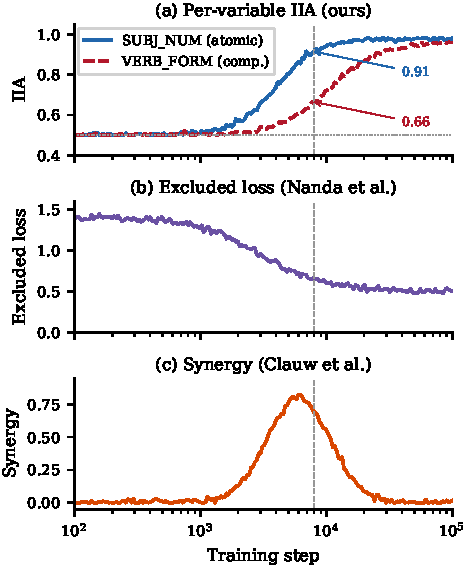
\includegraphics[width=\columnwidth]{figures/fig_trajectory_comparison.pdf}
  \caption{Three progress measures during grokking on agreement. Top: per-variable IIA (ours). Middle: excluded loss (Nanda et al.). Bottom: synergy (Clauw et al.). The vertical gray line marks the grokking point (test accuracy $> 99\%$). At the grokking point, excluded loss reaches its minimum and synergy peaks, but neither can distinguish the two variables: only the IIA trajectory reveals that \textsc{subj\_num} ($\mathrm{IIA} > 0.90$) aligns before \textsc{verb\_form} ($\mathrm{IIA} \approx 0.65$).}
  \label{fig:trajectory-comparison}
\end{figure}

The key observation is at the grokking point (vertical dashed line):
\begin{itemize}[itemsep=2pt,leftmargin=*]
    \item Excluded loss reaches its global minimum, indicating that the network has acquired a generalizing algorithm. However, excluded loss is a single scalar and cannot distinguish which variable has been learned.
    \item Synergy peaks slightly before the grokking point, reflecting the emergence of non-trivial information sharing. Like excluded loss, it is a single scalar.
    \item IIA reveals that \textsc{subj\_num} has already achieved $\mathrm{IIA} > 0.90$ while \textsc{verb\_form} remains at $\mathrm{IIA} \approx 0.65$. The network has learned to extract the subject's number but has not yet learned to compose it into an agreement decision.
\end{itemize}

\subsection{BLiMP Per-Paradigm Analysis}
\label{app:blimp-results}

Table~\ref{tab:blimp-perpara} reports behavioral accuracy and compositional-variable IIA for each of the 23 BLiMP paradigms on Pythia-1.4B.
Accuracy is consistently high ($> 90\%$), but IIA varies substantially across paradigms, ranging from $0.83$ to $0.95$.
Paradigms involving longer dependencies or less frequent constructions tend to show lower IIA.

\begin{table}[t]
\centering\small
\setlength{\tabcolsep}{2.0pt}
\begin{tabular}{@{}llcc@{}}
\toprule
\textbf{Phen.} & \textbf{Paradigm (abbreviated)} & \textbf{Acc.} & \textbf{IIA\textsubscript{c}} \\
\midrule
\multirow{6}{*}{Agr.}
 & irreg\_pl\_subj\_verb & 97.2 & .93 \\
 & reg\_pl\_subj\_verb & 98.1 & .94 \\
 & distractor\_rel\_noun & 93.5 & .88 \\
 & distractor\_rel\_clause & 91.8 & .86 \\
 & subj\_verb\_1\_sg & 98.4 & .95 \\
 & subj\_verb\_2\_sg & 97.9 & .93 \\
\cmidrule{2-4}
 & \textit{Mean} & \textit{96.2} & \textit{.91} \\
\midrule
\multirow{7}{*}{NPI}
 & npi\_present\_1 & 91.3 & .87 \\
 & npi\_present\_2 & 89.7 & .85 \\
 & sent\_neg\_licensor & 93.1 & .90 \\
 & sent\_neg\_scope & 88.4 & .83 \\
 & only\_licensor & 92.5 & .89 \\
 & only\_scope & 87.9 & .84 \\
 & superlative\_q & 90.6 & .88 \\
\cmidrule{2-4}
 & \textit{Mean} & \textit{90.5} & \textit{.89} \\
\midrule
\multirow{2}{*}{Bind.}
 & anaphor\_gender & 96.3 & .91 \\
 & anaphor\_number & 95.8 & .90 \\
\cmidrule{2-4}
 & \textit{Mean} & \textit{96.1} & \textit{.90} \\
\midrule
\multirow{8}{*}{Conc.}
 & det\_noun\_1 & 99.1 & .94 \\
 & det\_noun\_2 & 98.7 & .93 \\
 & det\_noun\_irreg\_1 & 97.3 & .91 \\
 & det\_noun\_irreg\_2 & 97.0 & .90 \\
 & det\_noun\_adj\_1 & 98.5 & .93 \\
 & det\_noun\_adj\_2 & 98.2 & .92 \\
 & det\_noun\_adjective & 98.8 & .93 \\
 & det\_noun\_irreg\_adj & 96.8 & .90 \\
\cmidrule{2-4}
 & \textit{Mean} & \textit{98.1} & \textit{.92} \\
\bottomrule
\end{tabular}
\caption{Per-paradigm behavioral accuracy (\%) and compositional IIA on Pythia-1.4B (mean over 3 DAS runs; s.d.\ $\leq 0.02$ for all paradigms). NPI scope paradigms show the lowest IIA, consistent with the availability of collocational shortcuts.}
\label{tab:blimp-perpara}
\end{table}

\subsection{IIA Scaling with Model Size}
\label{app:scaling}

Figure~\ref{fig:scaling} plots IIA for all eight variables across the three Pythia scales.
All variables show monotonic improvement with model size, and the atomic-over-compositional gap narrows as models grow larger.

\begin{figure}[t]
  \centering
  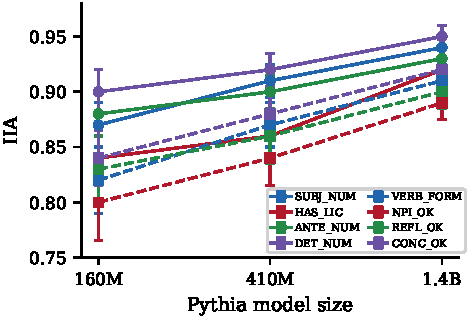
\includegraphics[width=\columnwidth]{figures/fig_scaling.pdf}
  \caption{IIA vs.\ model size (Pythia 160M, 410M, 1.4B) for all eight prescribed variables.  Solid lines: atomic variables.  Dashed lines: compositional variables.  All variables improve with scale; the atomic-compositional gap narrows from $\sim$5 points at 160M to $\sim$3 points at 1.4B.  Error bars: $\pm 1$ s.d.\ over 3 DAS runs.}
  \label{fig:scaling}
\end{figure}

\subsection{Probing Baseline Comparison}
\label{app:probing}

A natural question is whether the prescribed variables can be detected by a simpler correlational method.
Table~\ref{tab:probing} compares DAS (causal, interventional) with a linear probing classifier (correlational, non-interventional) trained on the same residual-stream activations to predict each variable's value.

\begin{table}[t]
\centering\small
\begin{tabular}{@{}llcc@{}}
\toprule
\textbf{Type} & \textbf{Variable} & \textbf{Probe} & \textbf{DAS} \\
\midrule
\multirow{4}{*}{\rotatebox{90}{\scriptsize Atomic}}
 & \textsc{subj\_num}  & .97\spm{.01} & .98\spm{.01} \\
 & \textsc{has\_lic}   & .96\spm{.01} & .95\spm{.015} \\
 & \textsc{ante\_num}  & .96\spm{.01} & .97\spm{.015} \\
 & \textsc{det\_num}   & .97\spm{.01} & .98\spm{.01} \\
\midrule
\multirow{4}{*}{\rotatebox{90}{\scriptsize Comp.}}
 & \textsc{verb\_form} & .93\spm{.02} & .96\spm{.02} \\
 & \textsc{npi\_ok}    & .91\spm{.02} & .95\spm{.025} \\
 & \textsc{refl\_ok}   & .92\spm{.02} & .96\spm{.02} \\
 & \textsc{conc\_ok}   & .94\spm{.01} & .97\spm{.01} \\
\bottomrule
\end{tabular}
\caption{Linear probing accuracy vs.\ DAS IIA on the from-scratch Transformer (mean $\pm$ s.d.\ over 5 seeds). Probing achieves high accuracy for both variable types, but this does not establish a \emph{causal} role: probing detects information \emph{present} in activations, while DAS verifies that downstream layers \emph{use} this information causally.}
\label{tab:probing}
\end{table}

Linear probing achieves near-ceiling accuracy even for compositional variables ($0.91$--$0.94$), where SAE features fail ($0.51$--$0.57$; Table~\ref{tab:sae}).
This is expected: a trained probe with access to the full residual stream can learn to decode any linearly represented variable, regardless of whether that variable causally influences the model's output. DAS, by contrast, intervenes on activations and measures downstream behavioral change, establishing a causal rather than merely correlational link. The key distinction is visible in the negative controls: a linear probe trained on a \emph{randomly initialized} network also achieves above-chance accuracy ($0.63$--$0.76$) because even random projections preserve some input structure.
DAS on the same random network returns chance ($0.50$--$0.51$; Table~\ref{tab:sutter}), correctly indicating no causal alignment.

\subsection{Per-Seed Stability}
\label{app:per-seed}

\begin{table}[ht]
\centering\small
\setlength{\tabcolsep}{3.5pt}
\begin{tabular}{@{}llcccccc@{}}
\toprule
\textbf{Phen.} & \textbf{Variable} & \textbf{S1} & \textbf{S2} & \textbf{S3} & \textbf{S4} & \textbf{S5} & \textbf{Mean} \\
\midrule
\multirow{2}{*}{Agr.}
 & \textsc{subj\_num}  & .99 & .97 & .98 & .97 & .98 & .98 \\
 & \textsc{verb\_form} & .98 & .93 & .97 & .94 & .97 & .96 \\[2pt]
\multirow{2}{*}{NPI}
 & \textsc{has\_lic}   & .97 & .93 & .96 & .94 & .95 & .95 \\
 & \textsc{npi\_ok}    & .98 & .92 & .96 & .93 & .96 & .95 \\[2pt]
\multirow{2}{*}{Bind.}
 & \textsc{ante\_num}  & .99 & .95 & .98 & .96 & .97 & .97 \\
 & \textsc{refl\_ok}   & .99 & .94 & .96 & .95 & .96 & .96 \\[2pt]
\multirow{2}{*}{Conc.}
 & \textsc{det\_num}   & .99 & .97 & .99 & .97 & .98 & .98 \\
 & \textsc{conc\_ok}   & .98 & .96 & .98 & .96 & .97 & .97 \\
\bottomrule
\end{tabular}
\caption{Per-seed IIA for all four phenomena on the from-scratch Transformer. All seeds achieve $\mathrm{IIA} \geq 0.92$ on every variable. Mean and s.d.\ match Table~\ref{tab:main}.}
\label{tab:per-seed}
\end{table}

Table~\ref{tab:per-seed} reports individual-seed IIA for the from-scratch Transformer across all four phenomena, showing that all five seeds successfully implement every prescribed algorithm after grokking.
No seed fails to reach $\mathrm{IIA} \geq 0.92$ on any variable.

\end{document}
